\documentclass{Vorlage}
%\usepackage[ngerman]{babel}
\usepackage{amsfonts}
\usepackage{graphicx}
\usepackage{url}
\usepackage{amsmath}
\usepackage{adjustbox}
\usepackage{color}
\usepackage{multirow}
\usepackage{bm}
\usepackage{cite}
\usepackage{subfigure}
%\usepackage[utf8]{inputenc}
%\bibliographystyle{apalike}
\setlength{\parindent}{0pt}
\usepackage{tabularx}

\pagestyle{fancy}
\renewcommand*\sectionmark[1]{\markboth{\MakeUppercase{#1}}{}}
\begin{document}

\newgeometry{top=2.5cm,bottom=2.0cm,left=2.5cm,right=2.5cm} % Befehl wird nur benötigt, falls Änderungen an den Seitenrändern in der Datei "Vorlage.cls" vorgenommen werden.

\begin{titlepage}

\begin{figure}
 \begin{center}
 
\includegraphics[scale=0.8]{Pictures/logo3}
 \end{center}
\end{figure}
\vspace*{3cm}




\titel{Kleinräumige Extrapolation von Umfragedaten}{}

\vspace{1cm}

\begin{tabular}{p{3.5cm}|p{0.1cm} p{10cm}l}
\textsc{Namen:} & & \textsc{Alexander Lange, Kai Husmann}\\
\textsc{Matr. Nr.:} & & \textsc{21426614, 20707176}\\
\textsc{Studiengang:} & & \textsc{Angewandte Statistik}\\
\textsc{Mail:} & & \textsc{Alexander.lange$ @ $stud.uni-goettingen.de}\\
\textsc{} & & \textsc{Kai.Husmann$ @ $forst.uni-goettingen.de}\\
\textsc{Kurs:} & & \textsc{Statistisches Praktikum}\\
\textsc{Kursleiter:} & & \textsc{Prof.Dr. Thomas Kneib}\\
\textsc{Lehrstuhl:} & & \textsc{Statistik}\\
\textsc{Fakultät:} & & \textsc{Wirtschaftswissenschaften}\\
\textsc{Abgabedatum:} & & \textsc{30. September 2016}\\
\end{tabular}
\end{titlepage}

\restoregeometry

\pagenumbering{Roman} % \pagenumbering{roman} = Kleinschreibung: II -> ii.

\pagestyle{plain}

\tableofcontents % Inhaltsverzeichnis.

\newpage % Neue Seite.

\listoffigures % Abbildungsverzeichnis.

\newpage

\listoftables % Tabellenverzeichnis.

\newpage

\pagenumbering{arabic} % Ab hier folgt die arabische Seitennummerierung.

%\renewcommand{\thesection}{\arabic{section}} % Römische Nummerierung der Kapitelüberschriften.

%============================================ Instroduction ========================================================%
\pagestyle{fancy}

\section{Einleitung}
Kleinräumige Extrapolation von Umfragedaten besitzt vor allem eine hohe Relevanz bei Städten, Kommunen und Gemeinden um städtische oder ländliche Planung auf wissenschaftlich fundierten Erkenntnissen voranzutreiben \cite{Planung}. Dabei kann die konkrete Fragestellung bzw. das Anwendungsgebiet sehr vielfältig sein. Es kann genutzt werden, um z.B. Landschaftsbilder nach den Vorstellungen und im Einvernehmen mit den Einwohnern einer Region zu Planen \cite{Natur}, oder um die Infrastruktur von Kommunen den Bedürfnissen der Bürger durch den demographischen Wandel anzupassen \cite{Lubeck}.\\
Bei einer kleinräumigen Extrapolation werden die Erkenntnisse einer Stichprobe auf die Grundgesamtheit dieser Stichprobe projiziert. Hierzu werden relevante Regeln und Eigenschaften der Stichprobe genutzt, um eine Variable von Interesse in die Grundgesamtheit zu prognostizieren, bei welcher diese Variablen nicht bekannt sind. Üblicherweise wird ein auf den Daten der Stichprobe basierendes Regressionsmodell parametrisiert und an der Grundgesamtheit angewendet. Mit diesem Ansatz werden im Wesentlichen zwei Ziele verfolgt. Einerseits werden durch die Extrapolation selbst neue, interessante Informationen über die Grundgesamtheit verfügbar ohne diese für jedes Individuum der Grundgesamtheit erheben zu müssen. Eine einfache deskriptive Auswertung der relevanten Variablen aus der Stichprobe führt zu verzerrten Schätzungen, wenn Gruppen über- oder unterrepräsentiert sind. Des Weiteren lassen sich aus den Regressionsmodellen häufig, beispielsweise durch Interpretation der Modellparameter oder der Modellintervalle, interessante Sekundärinformationen gewinnen. Kleinräumige Extrapolationen sind also eine effektive Methode um relevante Informationen, die nicht mit vertretbarem Aufwand bei einer Grundgesamtheit erhoben werden können, valide zu ergänzen.\\
Ziel dieser Arbeit ist es, kleinräumige Extrapolationen für zwei Beispiele in Stuttgart durchzuführen. Konkret geht es um die Extrapolation der Fragen: \textit{Wie ist die Meinung der Bürger Stuttgarts zum Projekt Stuttgart 21?} und \textit{Wie bewerten die Bürger Stuttgarts ihre Wohngegend?}. Dazu parametrisieren wir mithilfe einer Stichprobe, die ca. 0,05\% der Gesamtbevölkerung Stuttgarts umfasst geoadditive Regressionsmodelle und wenden diese an zwei Erhebungen mit deutlich größerem Stichprobenumfang an. Wir zeigen in dieser Arbeit, dass die Extrapolation mit diesen Modellen möglich und auch sinnvoll ist und warum die einfache deskriptive Auswertung der Stichprobe nicht zum gewünschten Ergebnis führt.\\
Dabei liegt der Schwerpunkt dieser Arbeit auf der Untersuchung verschiedener statistischer Methoden. Wir überprüfen, in welchen Fällen und in welcher Form räumliche Informationen und verschiedene Verteilungsannahmen zu einem Erkenntnisgewinn in Bezug auf die Fragestellungen führen. Hierzu wird eine Vielzahl additiver Modelle anhand mehrerer Evaluierungsmethoden geprüft. Am Ende steht eine fundierte Einschätzung über die vielversprechendsten Möglichkeit der Modellierung der beiden Fragestellungen.\\
\newpage

%=================================================== Main Part  ====================================================%
\section{Material und Methoden}
\subsection{Daten}
Insgesamt liegen für die Analysen drei Umfragen mit unterschiedlichen Stichprobenumfängen vor. Die kleinste Datei 
enthält Angaben zur Bewertung der Wohngegend, der Meinung zu Stutttgart 21 sowie weitere sozioökonomische Kovariablen, 
die zur Erklärung der beiden abhängigen Variablen dienen sollen. Sie wird im Folgenden als 
Parametrisierungsstichprobe bezeichnet. Die Parametrisierungsumfrage ist eine Stichprobe von 
der die Grundgesamtheit im strikteren Sinne für eine Validierung nicht zur Verfügung steht. Alle Modellqualitätskriterien müssen 
demnach entweder an der Stichprobe selbst oder an einer anderen Erhebung entwickelt werden. Die beiden anderen 
Umfragen haben jeweils einen deutlich größeren Stichprobenumfang. An diesen Umfragen werden die parametrisierten 
Modelle angewendet und die Meinung zu Stuttgart 21 sowie die Wohnzufriedenheit somit kleinräumig extrapoliert. Einige 
Variablen unterscheiden sich in ihren Ausprägungen zwischen den Umfragen. Zur Vereinheitlichung der Dateien mussten 
einige Gruppenausprägungen demnach umkodiert werden. Die Umkodierungen können in der digital anhängenden Datei 
\textit{Aufbereitung\_Stuttgart21.R} nachvollzogen werden.

\subsubsection{Parametrisierungsstichprobe}
Mit den Datensätzen der Parametrisierungsstichprobe (Tabelle \ref{Datensatz}) werden die Modelle für die kleinräumige 
Extrapolation parametrisiert. Bei dieser Umfrage handelt es sich um eine Befragung aus dem Jahr 2015 zur Lebensqualität 
der Einwohner Stuttgarts bei der unter anderem die Bewertung der Wohnsituation und die Meinung zu Stuttgart 21 abgefragt 
wurden \cite{Stuttgart2015}. Insgesamt standen 8 sozioökonomische Variablen und Angaben zur räumlichen Lage zur 
Verfügung. Von jedem Datensatz waren die stetige räumliche Lage als Gauß-Krüger Geokoordinate sowie die diskrete räumliche 
Lage im Stadtteil und Stadtbezirk bekannt.\\

\begin{table}[h]
\centering
\caption{Erhobene sozioökonomische und geographische Variablen der Parameterisierungsstichprobe und deren Anzahl der Ausprägungen sowie vermutete Modellierung im additiven Modell.}
\label{Datensatz}
\adjustbox{max height=\dimexpr\textheight-5.5cm\relax,
           max width=\textwidth}{
\begin{tabular}{l|c|c}
\multicolumn{2}{l}{Anzahl Beobachtungen: 3.143}     \\ \hline \hline
\textbf{Variable} & \textbf{Anzahl Ausprägungen} & \textbf{Modellierung} \\ \hline
Bewertung Wohngegend &  6 & Geordnet Kategorial \\ \hline
Meinung Stuttgart 21 &  6 & Geordnet Kategorial \\ \hline
Personenanzahl im Haushalt & 5 & Nicht Parametrisch \\ \hline
Monatliches Netto Haushaltseinkommen & 6 & Nicht Parametrisch \\ \hline
Altersklasse Befragter & 6 & Nicht Parametrisch \\ \hline
Geschlecht & 2 & Parametrisch\\ \hline
Familienstand & 4 & Parametrisch \\ \hline
Nationalität & 2 & Parametrisch \\ \hline
Stadtbezirk & 23 & Markov-Zufallsfeld \\ \hline 
Stadtteil &  142 & Markov-Zufallsfeld \\ \hline 
Gauß-Krüger & & Tensorprodukt-Splines  \\ \hline \hline
\end{tabular}
}
\end{table}

In Tabelle \ref{Datensatz} sind nicht nur die Anzahlen der Ausprägungen der Variablen, sondern auch die vermuteten 
Formen der Einflüsse der Kovariablen auf die abhängigen Variablen nach visueller Einschätzung aufgelistet. Es ist 
ersichtlich, dass alle nominal skalierten Variablen, wie z.B. die Nationalität, als parametrisch und dass 
alle kardinal skalierte Variablen, wie z.B. die Altersklasse des Befragten, als nicht-parametrisch 
modelliert werden sollten. Laut \cite[p.9]{fahrmeir2009regression} sind diese beobachteten Zusammenhänge typisch für 
eine Regressionsanalyse. In Anlehnung an \cite[p. 503 ff. \& p. 524 ff.]{fahrmeir2013regression} wird der 
kontinuierliche räumliche Effekt durch ein Tensor Produkt und die diskreten räumlichen Effekte durch ein Markov-Zufallsfeld im additiven Regressionsmodell berücksichtigt.\\
Für die Auswahl der geeigneten Regressionsmethode und der Ergebnisinterpretation ist es hilfreich, das Verhältnis der 
Häufigkeiten der Kategorienausprägungen der abhängigen Variable zu kennen und seltene Ereignisse zu identifizieren. 
Während die meisten befragten Personen ihre Wohngegend mit \textit{gut} oder \textit{sehr gut} bewertet haben, treten 
Beobachtungen mit \textit{schlechter} oder \textit{sehr schlechter} Einschätzung relativ selten auf (Tabelle 
\ref{endogene}). Im Vergleich sind die Verhältnisse der Gruppenhäufigkeiten zur Meinung zu Stuttgart 21 
ausgeglichener. Die \textit{neutrale} Haltung ist etwa halb so häufig vertreten wie die \textit{zustimmende} Haltung. 
Bei beiden Variablen wurden die wenigen, für die Modellierung irrelevanten, Kategorien 
\textit{Keine Angabe} entfernt. Den Variablen kann in bei der Gruppenausprägung eine Rangfolge, jedoch kein 
Intervall unterstellt werden. Es handelt sich demnach in beiden Fällen um ordinal Skalierte Daten.

\begin{figure}[h]
 \begin{center}
 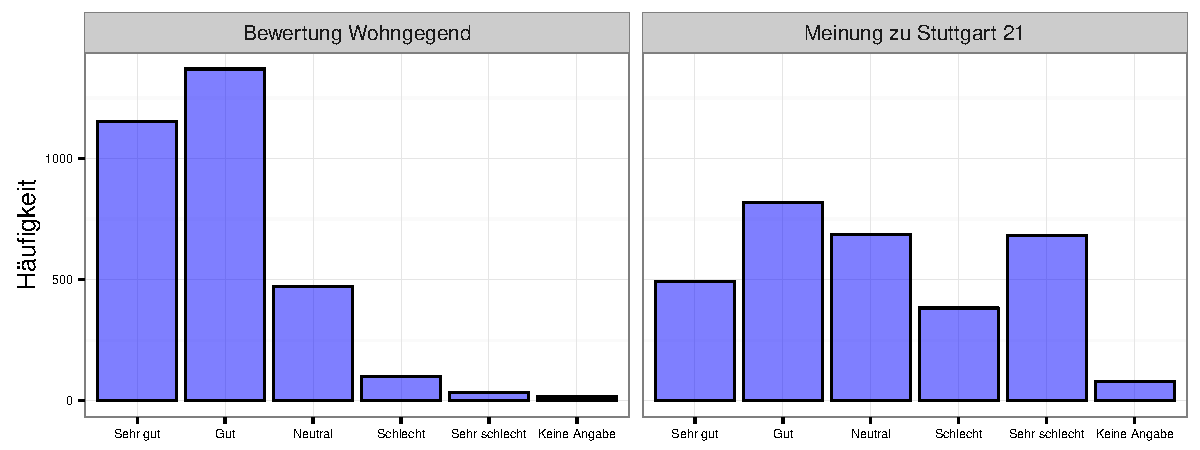
\includegraphics[scale=0.8]{Pictures/BarResp}
 \caption{Häufigkeit der Kategorienausprägungen der endogene Variablen in der Parameterisierungsstichprobe.}
 \label{endogene}
 \end{center}
\end{figure}

Das amtliche, nach Stadtteilen oder Stadtbezirken aufgelöste Ergebnis der Volksabstimmung zu Stuttgart 21 von 2011 kann 
dem Internetauftritt der Stadt entnommen werden \cite{Amt}. Es bietet sich dadurch eine zusätzliche Möglichkeit zur 
Modellevaluierung an, indem die Modellierungsergebnisse mit den tatsächlichen Ergebnissen verglichen werden. Da bei der 
Abstimmung mit Sicherheit nur die beiden Kategorien (\textit{Zustimmung} und \textit{Ablehnung }) unterschieden werden 
können, wurden die Gruppenausprägungen der Parameterisierungsstichprobe neu zusammengefasst. In den Rohdaten wurden noch 
sechs Gruppen unterschieden. Es wurde eine Neugruppierung in drei Gruppenausprägungen vorgenommen (Tabelle \ref{endogene}). Dafür wurden jeweils die 
Gruppen \textit{sehr gut} und \textit{gut} zu \textit{Zustimmung} und \textit{schlecht} und \textit{sehr schlecht} zu 
\textit{Ablehnung} zusammengefasst. Falls nur \textit{Zustimmung} und \textit{Ablehnung} für die Modellierung 
berücksichtigt werden sollen, reduziert sich der Stichprobenumfang auf 2377 Beobachtungen. Dadurch bleibt die 
Möglichkeit erhalten eine multinomial verteilte abhängige Variable zu modellieren und trotzdem eine Validierung für 
zwei Klassen vorzunehmen. Für die exogen in die Analyse einfließenden Variablen sind detailliertere Informationen zu den 
Häufigkeiten der Ausprägungen im Anhang verfügbar (Abbildung \ref{exogen_parametrisierungsdatensatz}). \\

Da in dieser Arbeit ein Schwerpunkt auf der Analyse unterschiedlicher räumlicher Effekte liegt, vergleicht dieser Abschnitt alle drei räumlichen Effekte in Bezug zu den beiden endogenen Variablen. Abbildung \ref{XYStuttgart3} zeigt die absolute Häufigkeit der Beobachtungen der Meinung zu Stuttgart 21 in kontinuierlicher räumlicher Lage. Zur besseren Übersicht wurden nicht alle Beobachtungen geplottet, sondern Beobachtungsdichten über bivariate normalverteilte Kerndichteschätzer mit festem Abstand für jede Richtungen ermittelt \cite{ggplot} sowie \cite{MASS}. Um die Hintergrundkarte einbinden zu können wurden die Gauß-Krüger Koordinaten in Dezimalgrad umgerechnet. Da absolute Dichten dargestellt werden, ist die Dichte der Kategorien nicht nur von der Anzahl der Kategorien selbst, sondern auch von der Einwohnerdichte beeinflusst. Des weiteren wird die Dichte von der Ausschöfung, also der Anzahl beantworteter Befragungsbögen beeinflusst. Wegen der hohen Einwohnerdichte im Innenstadtbereich sind dort die Beobachtungsdichten aller 3 Klassen tendenziell höher als in den Randbezirken. Des weiteren ersichtlich ist, dass einige Bereiche, wie das Naturschutzgebiet \textit{Rotwildpark} im Westen oder der \textit{Schurwald} im Osten, aufgrund ihrer geographischen Beschaffenheit oder Landnutzungsform nicht oder relativ dünn besiedelt sind.

\begin{figure}[h]
 \begin{center}
 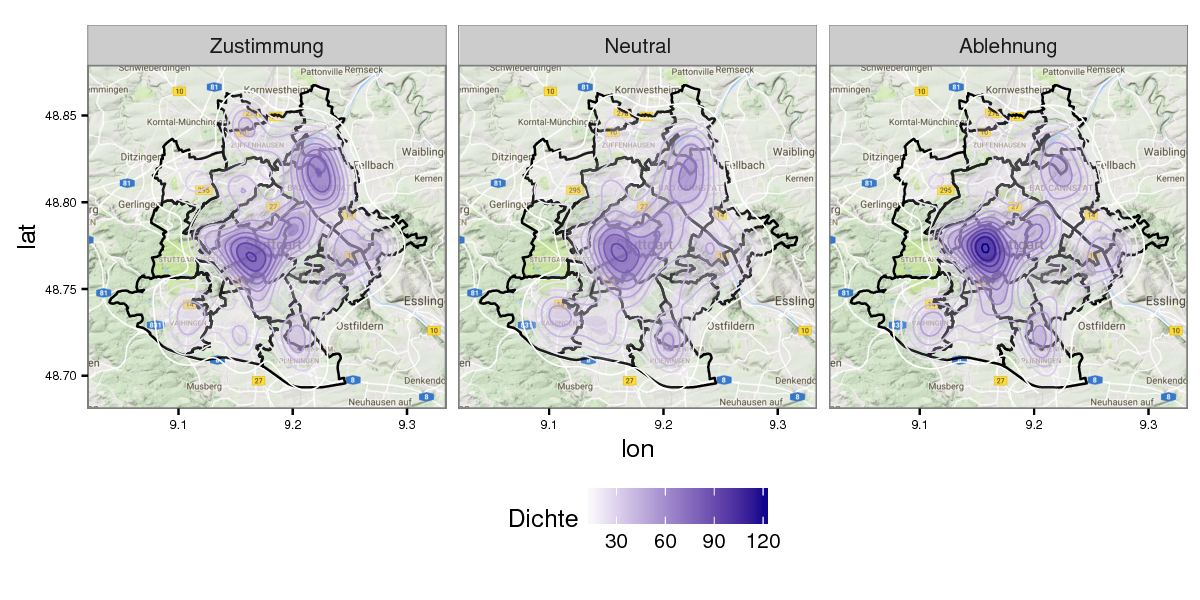
\includegraphics[scale=0.8]{Pictures/XYStuttgart3.png}
 \caption{Kontur Plot der absoluten Anzahl der Gruppenbeobachtungen zur Meinung zu Stuttgart 21 in drei Gruppen. Quelle der Hintergrundgrafik: \cite{google}}
 \label{XYStuttgart3}
 \end{center}
\end{figure}

Die \textit{Zustimmung} zeigt offensichtliche räumliche Muster. Im Zentrum und im Nordosten ist sie höher als im Rest 
der Stadt. Der räumliche Trend der \textit{Ablehnung} ist schwächer ausgeprägt. Es zeigt sich jedoch, dass der Bereich 
der Innenstadt, sowie die südlichen Stadtbereiche etwas höhere Dichten bei der \textit{Ablehnung} aufweisen. Die 
Beobachtungen der Kategorie \textit{neutral} sind eher gleichmäßig über die Stadt verteilt.\\
Abbildung \ref{XYWohnG5} zeigt die Dichte der Beobachtungen der fünf Kategorien zur Bewertung der Wohngegend. Hier zeigt sich ein deutlich ausgeprägteres räumliches Muster als bei der Meinung zu Stuttgart 21. Die Beobachtungen der Klasse \textit{sehr gut} häufen sich sehr stark im Innenstadtbereich und im Süden. Die Kategorie \textit{gut} verteilt sich relativ homogen über das gesamte Stadtgebiet mit einer etwas stärkeren Konzentration in der Innenstadt und im Nordosten. Bei der Klasse \textit{neutral} zeigt sich eine stärkere Konzentration auf den Osten und Nordosten der Stadt. Praktisch alle \textit{schlechten} und \textit{sehr schlechten} Bewertungen sind deutlich abgegrenzt im Osten und Nordosten lokalisiert. Hierbei ist zu erwähnen, dass der Anteil der Personen, die ihre Wohngegend mit \textit{schlecht} oder \textit{sehr schlecht} bewertet haben sehr gering ist Abbildung \ref{endogene}.\\

\begin{figure}[h]
 \begin{center}
 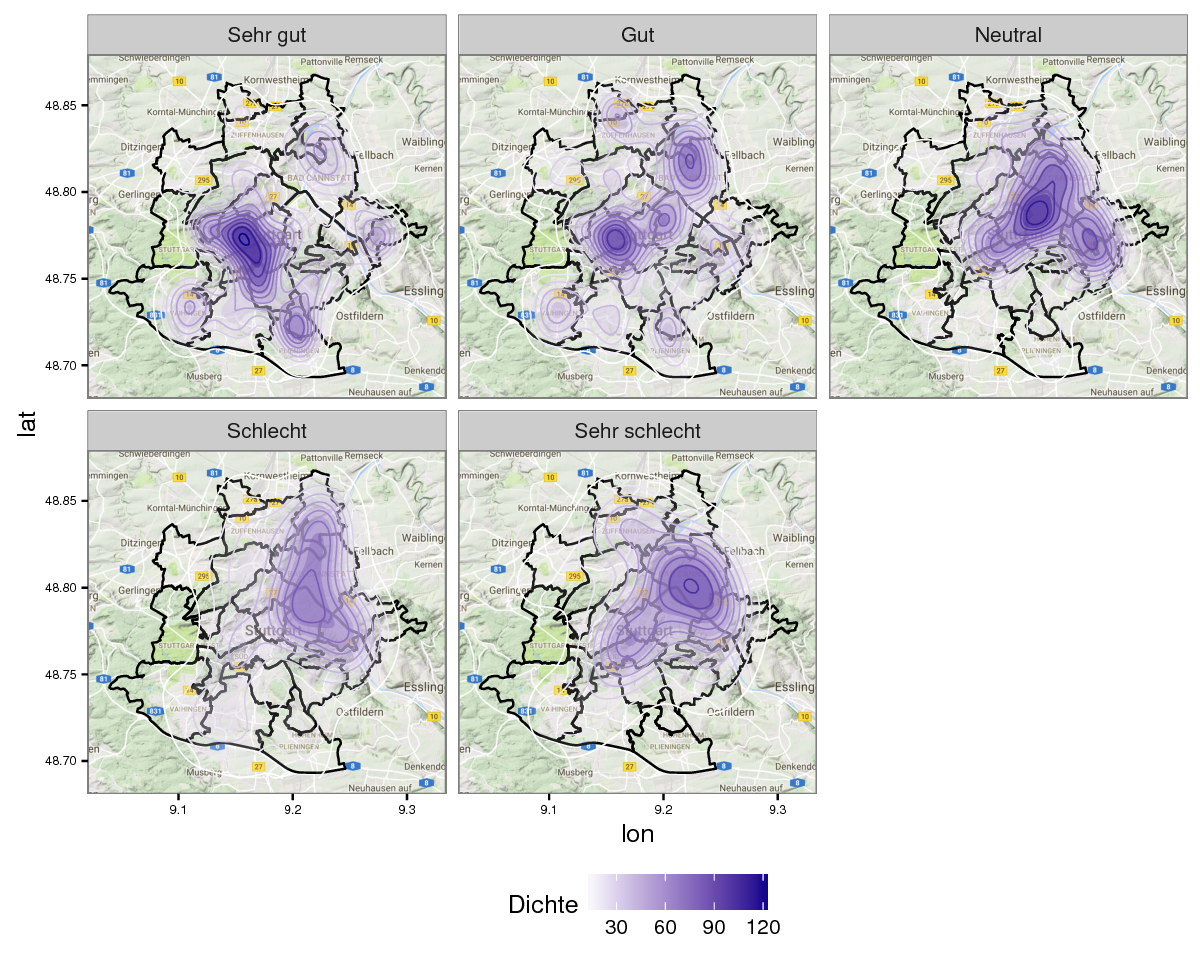
\includegraphics[scale=0.8]{Pictures/XYWohnG5.png}
 \caption{Kontur Plot der absoluten Anzahl der Gruppenbeobachtungen zur Wohnzufriedenheit in fünf Gruppen. Quelle der Hintergrundgrafik: \cite{google}}
 \label{XYWohnG5}
 \end{center}
\end{figure}


Im folgenden werden die diskreten räumlichen Informationen auf Stadtbezirksebene beschrieben. Es werden 23 Stadtbezirke 
unterschieden. Im Gegensatz zur stetigen Beobachtungsdichte werden die Beobachtungen nach Regionen aggregiert 
dargestellt. Dies hat den Vorteil, dass eine relative Anteilsdarstellung möglich wird (Abbildung 
\ref{BStuttgart21}). Die absoluten Häufigkeiten sind jedoch nicht dargestellt. Analog zur stetigen Darstellung 
(Abbildung \ref{XYStuttgart3}) ist auch hier zu sehen, dass die Bürger des Nordostens eine positivere Meinung zu 
Stuttgart 21 haben als die Bürger aus dem Süden. Die \textit{neutrale} Klasse hat in allen Bezirken einen geringeren 
Anteil und es ist kein räumliches Muster erkennbar. Die entsprechenden Anteilsgrafiken mit fünf Klassen für die 
Bewertung der Wohngegend sind im Anhang verfügbar (Abbildung \ref{BWohn}). Wie in Abbildung \ref{XYWohnG5} bereits 
angedeutet, zeigen sich negative Wohngebietseinschätzungen vor allem im Nordosten.

\begin{figure}[h]
 \begin{center}
 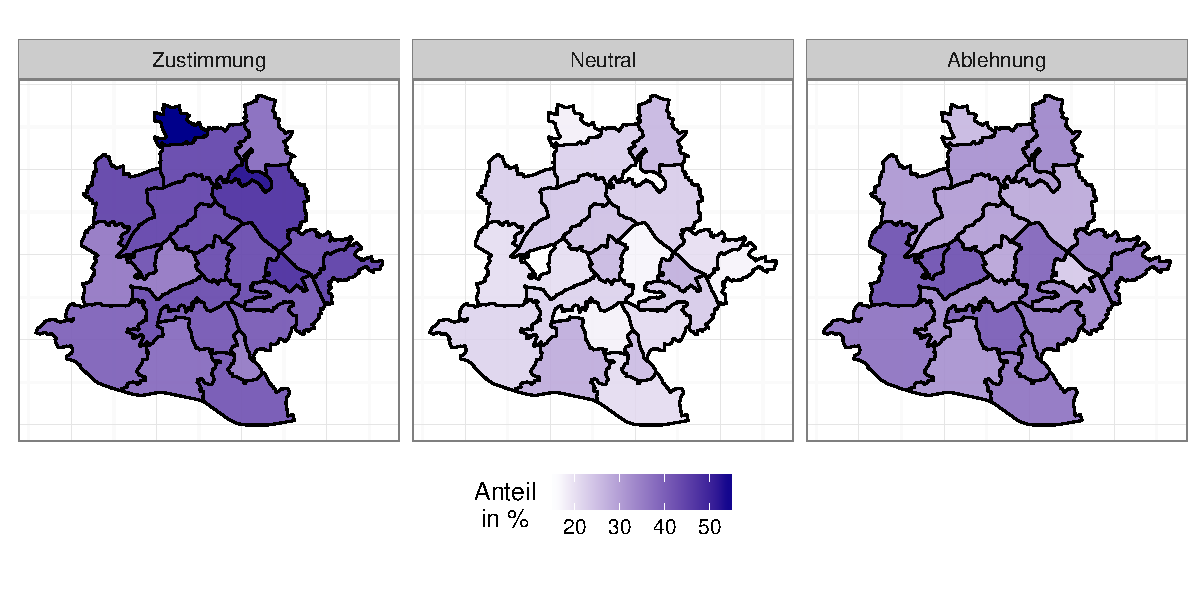
\includegraphics[scale=0.8]{Pictures/BStuttgart3}
 \caption{Anteile zur Meinung zu Stuttgart 21 nach Stadtbezirken.}
 \label{BStuttgart21}
 \end{center}
\end{figure}

Die dritte und letzte untersuchte räumliche Agrregationsebene ist die Stadtteilebene. Abbildung \ref{SStuttgart21} 
zeigt die räumliche Verteilung von \textit{Zustimmung}, \textit{Ablehnung} und \textit{neutraler} Haltung. Wie aus 
Tabelle \ref{Datensatz} hervorgeht, ist die Stadtteilebene deutlich feiner Aufgelöst als die Bezirksebene. Dies führt in 
der Abbildung dazu, dass einige Stadtteile mit geringer Gesamteinwohneranzahl in einer oder mehreren Klassen keine 
Beobachtungen zeigen. Es gibt im Umkehrschluss auch Stadtteile, in denen eine Klasse zu 100 \% vertreten ist. 
Außerdem gibt es in dieser Aggregationsebene sogar Stadtteile ohne jede Beobachtung, wie z. B. das Benzviertel im 
Innenstadtbereich oder die bereits angesprochenen Lagen im Westen.

\begin{figure}[h]
 \begin{center}
 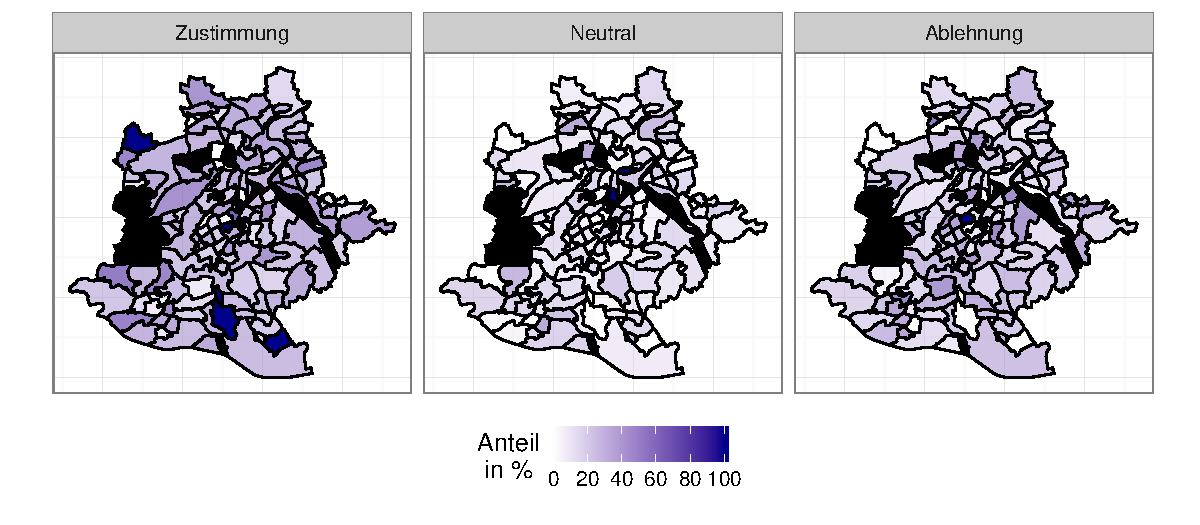
\includegraphics[scale=0.8]{Pictures/SStuttgart3}
 \caption{Anteile der Meinung zu Stuttgart 21 nach Stadtteilen.}
 \label{SStuttgart21}
 \end{center}
\end{figure}

Diese Stadtteile werden in den Diagrammen schwarz dargestellt. Wegen der feineren Auflösung ergibt sich ein 
mosaikartiges, visuell schwerer interpretierbares Bild. In keiner der drei Klassen lässt sich eine klare Struktur oder 
ein räumliches Muster erkennen. Die Anteile auf Stadtteileebene zu der Bewertung der Wohngegend sind im Anhang 
verfügbar \ref{SWohn}. Hier zeigt sich ein ähnlich schwer differenzierbares Muster wie bei der Meinung zu Stuttgart 21. 
Wegen der deutlichen Unterschiede in den Anteilen der fünf Gruppen sind die Farbskalen nicht einheitlich, sondern 
unterscheiden sich in den Diagrammen.\\

\subsubsection{Melderegister}
Die erste Datei an der die Modelle Anwendung finden sollen ist eine personenbezogene Auswertung aus dem Melderegister 
Stuttgarts vom 31.01.2011. Der Auszug umfasst alle volljährigen Einwohner Stuttgarts außer Bewohner von Anstalten und 
Pflegeheimen. Mit einem Stichprobenumfang von 470.190 Bürgern liegt der Melderegisterauszug also sehr nah an 
der Grundgesamtheit von 573.104 Bürgern, die 2011 mit Hauptwohnsitz in Stuttgart gemeldet waren \cite{bundesamt}. Insgesamt wurden acht sozioökonomische Variablen erhoben. Bei allen Datensätzen liegt der Wohnsitz als 
kontinuierliche Gauß-Krüger Geokoordinate vor. Um eine kleinräumige Extrapolation mit diskreten räumlichen 
Informationen vornehmen zu können, wurden die Stadtteil- und Stadtbezirksinformationen an die Datensätze des 
Melderegisters angehängt. Hierzu wurden die Stadtteil- und Stadtbezirkspolygone, welche uns von der Stadt Stuttgart für 
die Analyse zur Verfügung gestellt wurden, über eine räumliche Abfrage mit den Melderegisterdatensätzen verknüpft. Die 
geographische Verknüpfung wurde mit dem freien Geoinformationssystem QGIS \cite{qgis2016} durchgeführt. Die 
Projektdatei mit der Geoabfrage (\textit{Geographische\_Abfrage.QGS}) sowie die Shapefiledateien 
(\textit{Stadtteile\_netto.SHP}) liegen dieser Arbeit digital bei. Wie in den Tabellen \ref{Datensatz} und 
\ref{Var_Buergerumfrage} ersichtlich, eignen sich nicht alle Variablen zur Extrapolation, da nicht alle Variablen in 
jeder Umfrage erhoben wurden. Es ergibt sich ein Überschneidungsbereich der fünf sozioökonomischen Variablen 
\textit{Altersklasse Befragter}, \textit{Geschlecht}, \textit{Nationalität}, \textit{Familienstand} und 
\textit{Personenzahl im Haushalt} enthält. Die Variablenkategorien wurden zum Teil umkodiert, um gleiche Ausprägungen in allen Dateien zu gewährleisten.

\begin{table}[h]
\centering
\caption{Sozioökonomische und geographische Variablen des Melderegisters und deren Anzahl der Ausprägungen.}
\label{Var_Buergerumfrage}
\adjustbox{max height=\dimexpr\textheight-5.5cm\relax,
           max width=\textwidth}{
\begin{tabular}{l|c}
\multicolumn{2}{l}{Anzahl Beobachtungen: 470.190}     \\ 
\hline \hline
\textbf{Variable}  & \textbf{Anzahl Ausprägungen}  \\ \hline
\multicolumn{1}{l|}{Altersklasse Befragter}  & 6 \\ \hline
\multicolumn{1}{l|}{Geschlecht}   & 2 \\ \hline
\multicolumn{1}{l|}{Nationalität}   & 2 \\ \hline
\multicolumn{1}{l|}{Familienstand}  & 4 \\ \hline
\multicolumn{1}{l|}{Personenzahl im Haushalt}   & 5 \\ \hline
\multicolumn{1}{l|}{Wohndauer}   & 3 \\ \hline
\multicolumn{1}{l|}{ALG II Quote}   & 9 \\ \hline
\multicolumn{1}{l|}{Ein/Zweifamilienhäuser} & 8 \\ \hline 
\multicolumn{1}{l|}{Gauß-Krüger}  & \\ \hline \hline
\end{tabular}

}
\end{table}

\subsubsection{Zensus}
Im Rahmen der bundesweiten Volkszählung von 2011 wurde in Stuttgart eine Gebäude- und Wohnungszählung durchgeführt. Diese Datei umfasst 380.238 Bürger Datensätze (Tabelle \ref{Var_Zensus}). Da bei der Zählung auch für die Fragestellung dieser Arbeit relevante sozioökonomische Variablen 
erhoben wurden, eignet sich diese Umfrage ebenfalls zur kleinräumige Extrapolation. Die diskreten geographischen 
Angaben wurden analog zum Vorgehen beim Melderegister per geographischer Abfrage ergänzt. Für die kleinräumige Extrapolation kommen 
die gleichen sozioökonomischen Variablen wie beim Melderegister in Frage. 

\begin{table}[h]
\centering
\caption{Sozioökonomische und geographische Variablen der Gebäude- und Wohnungszählung im Rahmen des Zensus und deren Anzahl der Ausprägungen.}
\label{Var_Zensus}
\adjustbox{max height=\dimexpr\textheight-5.5cm\relax,
           max width=\textwidth}{
\begin{tabular}{l|c}
\multicolumn{2}{l}{Anzahl Beobachtungen: 380.238}     \\ 
\hline \hline
\textbf{Variable}  & \textbf{Mögliche Ausprägungen}  \\ \hline
\multicolumn{1}{l|}{Altersklasse Befragter} &   6 \\ \hline
\multicolumn{1}{l|}{Geschlecht} &  2 \\ \hline
\multicolumn{1}{l|}{Nationalität} &  2 \\ \hline
\multicolumn{1}{l|}{Familienstand} & 4 \\ \hline
\multicolumn{1}{l|}{Personenzahl im Haushalt}   & 5 \\ \hline
\multicolumn{1}{l|}{Wohnfläche} & 24 \\ \hline
\multicolumn{1}{l|}{Stellung Beruf}   & 9 \\ \hline
\multicolumn{1}{l|}{Beamter} & 2 \\ \hline 
\multicolumn{1}{l|}{Gebäudetyp} & 10 \\ \hline
\multicolumn{1}{l|}{Gebäudenutzung} & 2 \\ \hline
\multicolumn{1}{l|}{Gauß-Krüger}  & \\ \hline \hline
\end{tabular}

}
\end{table}

\newpage

\subsection{Statistische Methoden}

Zur Vorstellung der statistischen Methoden dieser Arbeit wird zunächst das Verfahren zur Wahl der Kovariablen in jedem Modell erläutert. Anschließend folgt eine Darstellung des Geoadditiven Modells, welches zur Parametrisierung und anschließenden Extrapolation genutzt wird. Dabei wird insbesondere auf die modelspezifischen Besonderheiten der endogenen Variablen eingegangen, sowie auf die Modellierung der unterschiedlichen Kovariablen, die im vorangegangen Kapitel erläutert wurden. Außerdem wird kurz auf die Implementierung am Rechner eingegangen. Anschließend erfolgt eine Darstellung der Methoden, die zur Ermittlung des jeweils besten Modells für beide endogene Variablen genutzt werden. Dabei wird unterschieden zwischen der Modellqualität innerhalb und außerhalb der Stichprobe. Sämtliche Berechnungen wurden mit Hilfe der Statistik Software \texttt{R} vorgenommen \cite{RCore}.

\subsubsection{Schrittweiser AIC Vergleich}
Basierend auf den vorhergegangenen Analysen des Beamten- und Eigenheimanteils in Stuttgart, die uns zur Verfügung standen wurde eine Funktion zur schrittweisen AIC \cite{Akaike1981} Berechnung programmiert, die zur Identifikation der geeignetsten sozioökonomischen Kovariablenkombination dient (siehe digitaler Anhang \textit{stepAIC.R}). In der Funktion werden mithilfe der \texttt{gam()} Funktion des \texttt{mgcv} 
Paketes \cite{Wood2011} generaliserte additive Modelle mit unterschiedlichen Kovariablen erstellt und deren AIC 
berechnet. Vor dem Aufruf der Funktion müssen die abhängige Variable, die Verteilungsannahme des Regressionsmodelles, 
die Gewichtungen der Einzelbeobachtungen und unveränderliche Kovariablen definiert werden. Außerdem muss eingeschätzt 
werden, welche der veränderlichen Kovariablen parametrisch oder semiparametrisch als Spline in das Modell eingehen. Es 
wird zunächst der AIC des einfachsten, nur aus den fest vorgegebenen Kovariablen bestehenden Modells berechnet. In 
Iteration eins werden alle veränderlichen Kovariablen einzeln nacheinander in die Modellformel aufgenommen und es wird 
jeweils ein GAM erstellt sowie dessen AIC berechnet. Die Kovariablen gehen zunächst entsprechend der vorigen Eingabe parametrisch 
oder semiparametrisch ein. Außerdem werden alle vorab als nichtparametrisch eingeschätzten Variablen zusätzlich als parametrischer Trend geprüft. Falls die Hinzunahme mindestens einer Kovariable in Iteration eins zu einer Reduktion des AIC 
führt, wird diejenige Kovariable, welche zu dem Modell mit dem kleinsten AIC führt zur Modellformel hinzugefügt. Falls 
das Modell nur mit den festen Modellbestandteilen bereits den geringsten AIC zeigt ist die Modellwahl folglich in 
Iteration eins bereits beendet.\\ 
Andernfalls setzt sich das Ausgangsmodell für Iteration zwei aus den festen 
Kovariablen und einer weiteren Kovariable zusammen. In Iteration zwei werden wie zuvor alle verbleibenden Kovariablen 
zunächst nacheinander zur aktuellen Modellformel hinzugefügt. Wenn die Kovariable mit dem geringsten AIC gefunden ist 
(falls diese existiert und das Modell aus Iteration eins nicht bereits das geeignetste ist), werden alle veränderbaren 
Kovariablen in Iteration zwei nochmals nacheinander eliminiert. Das Modell mit dem geringsten AIC bildet das 
Ausgangsmodell der nächsten Iteration. Dies wird wiederholt bis in einer Iteration kein Modell mit einem geringeren AIC 
als in der vorigen Iteration parametrisiert werden kann. Um die Laufzeit der Funktion zu begrenzen, wurde auf die 
Analyse von Wechselwirkungen zwischen den Kovariablen verzichtet. Wechselwirkungen können jedoch als unveränderliche 
Modellbestandteile eingehen. In dieser Arbeit wird der Einfluss unterschiedlicher räumlicher Effekte auf die Modellqualität analysiert. Die räumlichen Effekte wurden deshalb im schrittweisen AIC Vergleich nicht berücksichtigt. Sie gingen, sofern das betrachtete Modell über einen räumlichen Effekt verfügte, als unveränderlicher Modellbestandteil ein.

\subsubsection{Modelle}
Alle zu modellierenden endogenen Variablen besitzen kategoriale Merkmale. Ziel der Modellierung ist also  die Ausprägungswahrscheinlichkeit dieser Kategorien vorherzusagen. Da negative Wahrscheinlichkeiten sowie Wahrscheinlichkeiten über 1 nicht sinnvoll interpretierbar sind, muss demnach sichergestellt sein, dass die endogene Variable des Regressionsmodells nur stetige Werte zwischen 0 und 1 einnehmen kann. Da sich diese Vorgabe mit einfachen linearen Regressionsmodellen normalerweise nicht einhalten lässt, sind diese folglich für die Fragestellung dieser Arbeit ungeeignet. Des Weiteren weisen kategoriale Regressionsmodelle häufig keine Normalverteilung auf \cite[p. 277]{fahrmeir2013regression}, was zusätzlich gegen einfache lineare Modelle mit gewöhnlicher kleinste-Quadrate-Schätzung spricht. Im Gegensatz zu einfachen linearen Regression kann der lineare Prädiktor

\begin{equation} \label{linPraed}
\eta_{i} =\mathbf{x}'_i \boldsymbol{\beta},
\end{equation}

in generalisierten linearen Modellen (GLM) über eine Response-Funktion $h$ transformiert werden. Die Response-Variable hängt demnach nicht mehr direkt von einer linearen Kombination der Modellkovariablen, sondern von deren Transformation ab. Die Wahl der Response-Funktion hängt von der Fragestellung und von der Skalierung der Response-Variable ab. $h$ kann jede monoton ansteigende Funktion sein. Um den gewünschten Wertebereich zwischen 0 und 1 sicherzustellen wird der lineare Prädiktor bei kategorialen Regressionen häufig über eine logistische Response-Funktion transformiert. Im Falle einer binären Response-Variable ergibt sich durch die logistische Transformation nach \cite[p. 270 f.]{fahrmeir2013regression} das binäre Logit Modell

\begin{equation} \label{logit}
h(\eta)=\frac{\exp(\eta)}{1+\exp(\eta)},
\end{equation}

wobei die Response nach der Transformation einer Bernoulli Verteilung folgt. Durch Datengruppierung kann die Rechenzeit reduziert werden. Die absoluten Gruppenhäufigkeiten folgen dann einer Binomial- und die relativen Gruppenhäufigkeiten skalierten Binomialverteilungen \cite[p. 277 f.]{fahrmeir2013regression}.\\
In einem kumulativen Modell kann die Reihenfolge der Ausprägungen einer ordinalskalierten Response explizit berücksichtigt werden \cite[p.334 ff.]{fahrmeir2013regression}. Dem kumulativen Modell unterliegt die Annahme, dass in jedem Datensatz eine kontinuierliche (unbekannte) latente Variable $u_i$ existiert, deren Ausprägung die Kategoriezugehörigkeit dieser Beobachtung bestimmt. Dem Modell unterliegt des Weiteren die Annahme, dass diese latente Variable durch einen linearen Prädiktor

\begin{equation}
u_i=-\mathbf{x}'_i \boldsymbol{\tilde{\beta}}+\varepsilon,
\end{equation}

über die Modellkovariablen vorhergesagt werden kann. Ein Datensatz zeigt die Ausprägung $r$, wenn ihre latente Variable zwischen den Schwellenwerten $\theta_{r-1}$ und $\theta_r$ liegt. Um sicherzustellen, dass diese Schwellenwerte identifizierbar sind, hat der lineare Prädiktor selbst keinen Intercept. Wie zuvor im binären Fall, wird der lineare Prädiktor über eine kumulative Verteilungsfunktion transformiert. Über die Verteilung $F$ des Fehlers des linearen Prädiktors  $\varepsilon_i$ um die latente Variable $u_i$ kann die Wahrscheinlichkeit jeder Kategorie der Response-Variablen als 

\begin{equation}
P(y_i=r)=F(\theta_r+\mathbf{x}'_i \boldsymbol{\tilde{\beta}})-F(\theta_{r-1}+\mathbf{x}'_i \boldsymbol{\tilde{\beta}})
\end{equation}

berechnet werden. Da es sich um geordnete Kategorien handelt, muss zur Berechnung der Wahrscheinlichkeit der Zugehörigkeit zur Gruppe $r$ nur die Wahrscheinlichkeitsdichte zwischen den Schwellenwerten $\theta_{r}$ und $\theta_{r-1}$ berechnet werden. Wenn die in der Literatur vorgeschlagene logistische Transformation gewählt wird \cite[p. 335]{fahrmeir2013regression}, ergibt sich demnach das kumulative Logit Modell

\begin{equation}
P(y_i\leq r)=\frac{\exp(\theta_r+\mathbf{x}'_i \boldsymbol{\tilde{\beta}})}{\exp(1+\exp(\theta_r+\mathbf{x}'_i \boldsymbol{\tilde{\beta}}))}.
\end{equation}

Die exogenen Variablen, mit denen das Modell für die räumliche Extrapolation parametrisiert werden soll, sind sehr heterogen. Es kommen sowohl nominal- als auch kardinalskalierte sozioökonomischen Variablen in Frage (Abbildung \ref{endogene}, Tabelle \ref{Datensatz}). Während ein linearer Prädiktor zur Beschreibung des Zusammenhangs zwischen ordinalskalierten Kovariablen und kategorieller Response-Variablen ausreichend ist, zeigen kardinal skalierte Variablen oft einen nichtlinearen Zusammenhang \cite[p. 9]{fahrmeir2009regression}. Der in generalisierten linearen Modellen (GLM) vorausgesetzte lineare Prädiktor (Formel \ref{linPraed}) ist demnach für die Daten dieser Arbeit zu unflexibel. Aufgrund dieser Ausgangslage haben flexiblere Modelle voraussichtlich Vorteile gegenüber GLM.\\
In generalisierten additiven Modellen (GAM) können lineare und nichtlineare Effekte sehr flexibel in einem Modell verbunden werden, da die Terme des Prädiktors in GAM nicht auf lineare Funktionen beschränkt sind (Formel \ref{SplinePraed}). Während die Kovariablen mit linearen Effekten $\mathbf{x}_i$, analog zum GLM, durch den linearen Prädiktor modelliert werden, können die nichtlinearen Kovariableneffekte $\mathbf{z}_i$ über sehr flexible, semi- bzw. nichtparametrische Splines modelliert werden \cite[p. 1 f.]{wood2016}. Obwohl die Formulierung \textit{nicht-parametrisch} für den in dieser Arbeit verwendeten Spline-Typ mathematisch unpräzise ist \cite[p. 1]{eilers1996}, wird sie, wie in der Literatur üblich, synonym für \textit{semiparametrisch} verwendet.

\begin{equation} \label{SplinePraed}
\eta_{i} =\mathbf{x}'_i \boldsymbol{\beta}+f_{i}(\mathbf{z}_{i})
\end{equation}

GAM bieten sich also immer an, wenn lineare und nichtlineare Kovariableneffekte in einem Modell berücksichtigt werden sollen oder wenn die genauen Formen der Effekte unbekannt sind. Zur Modellierung der univariaten nichtlinearen Effekte dieser Arbeit wurden penalisierte Basissplines (P-Splines) verwendet \cite{eilers1996}. Dieser Spline-Typ ist der Gruppe der semiparametrischen Modelle zuzuordnen, da die Spline-Kurve, im Gegensatz zu z. B. Kernel-Regressionen, über zusammengesetzte Polynome konstruiert wird. Das Modell setzt sich also aus einer großen Zahl abstrakter Variablen zusammen, die keine direkte Interpretation zulassen \cite[p. 1]{eilers1996}. Basissplines (B-Splines) haben gegenüber anderen Spline-Typen, wie z. B. \textit{Truncated-Power-Series-Basis-Splines}, numerische Vorteile da die Regressionsparameter relativ kleine Werte annehmen und die abschnittsweisen Polynome untereinander weniger stark korrelliert sind \cite[p. 426]{fahrmeir2013regression}. B-Splines können über die Methode der kleinsten Quadrate gelöst werden \cite[p. 430]{fahrmeir2013regression} und benötigen daher verhältnismäßig wenig Rechenzeit. Die Qualität der Anpassung eines polynomischen Splines hängt maßgeblich von Anzahl und Lage der Übergänge (Knoten) der zusammengesetzten Polynome ab. Hier liegt ein weiterer Vorteil der B-Splines. Während die optimale Glättung bei anderen Spline-Typen zum Teil aufwendig über Modellauswahlstrategien hergeleitet werden muss, kann bei B-Splines eine relativ simple Penalisierung definiert werden \cite[p. 89 f.]{eilers1996}. Hierzu wird zunächst ein sehr flexibles Modell mit einer großen Anzahl Spline-Basen definiert, welches ex-post über den Penalisierungsterm geglättet wird. Die Krümmung von zweifach differenzierbaren Funktionen kann über das Integral der zweiten Ableitung ermittelt werden. Bei B-Splines kann dieses Integral einfach über die quadrierten zweiten Abweichungen der Spline Funktion approximiert werden \cite[p. 433]{fahrmeir2013regression}. Die penalisierte Spline Kurve (P-Spline) kann daher über die penalisierte Methode der kleinsten Quadrate geschätzt werden. In die Schätzung gehen nur die Rohdaten und der Glättungsparameter $\lambda$ ein \cite[p. 93]{eilers1996}. Über $\lambda$ kann der Trade-Off zwischen Glättung und Anpassung eingestellt werden. Das R Paket \texttt{mgcv} \cite{Wood2011} liefert zudem unterschiedliche Möglichkeiten $\lambda$ auf Grundlage der Eingangsdaten, z. B. per \textit{generalisierter Kreuzvalidierung} \cite[p. 480]{fahrmeir2013regression} oder \textit{Restricted Maximum Likelihood} \cite[p. 32 f.]{wood2016}, zu optimieren. P-Splines sind demnach sehr komfortabel anzuwenden da sie außer den Eingangsdaten keine Benutzereingaben erfordern und die Rechenzeit gering ist.\\
Analog zu GLM können in GAM ebenfalls Response-Funktionen und unterschiedliche Verteilungsannahmen der Response Variablen definiert werden \cite[p. 448]{fahrmeir2013regression}. Die Ausprägungswahrscheinlichkeiten für binäre Responses können in GAM demnach über eine logistische Response-Funktion (Formel \ref{logit}) modelliert werden. Unterschiedlich ist lediglich der Prädiktor (Formel \ref{SplinePraed}). Eben dies gilt für geordnete kategoriale Modelle. Als kumulative Verteilungsfunktion für Wahrscheinlichkeitsdichte $F$ ist im \texttt{mgcv} Paket ebenfalls die logistische Transformationsfunktion implementiert \cite[p. 22]{wood2016}. In einem geordneten kategorialen GAM, das mit dem \texttt{mgcv}-Paket geschätzt wird, muss der erste \textit{Cutpoint} -1 sein \cite[p. 22]{wood2016}. Daher können die Prädiktoren von GAM, im Gegensatz zu einem GLM, einen Intercept haben.\\
Bei räumlich expliziten Daten kann häufig nicht von der Unabhängigkeit der Beobachtungen ausgegangen werden. Wie die visuelle Interpretation der Rohdaten nahelegt (z. B. Abbildung \ref{BStuttgart21}) zeigen räumlich nähere Beobachtungen mit höherer Wahrscheinlichkeit die gleiche Ausprägung als weiter entfernte. Es existiert offensichtlich räumliche Korrelation in den Daten. Das Modell lässt sich also voraussichtlich durch Hinzunahme eines räumlichen Effekts verbessern. Wenn in einem GAM räumliche Effekte berücksichtigt werden, spricht man von einem geoadditiven Modellen \cite[p. 540]{fahrmeir2013regression}. In dieser Arbeit wurden zwei unterschiedliche Methoden zur Berücksichtigung des räumlichen Effektes verwendet. Zunächst gingen die Gauß-Krüger Geokoordinaten $s_x$ und $s_y$ kontinuierlich in Form eines penalisierten \textit{Tensorprodukt Thin Plate Splines} (TP-Spline) ein. Diese Spline Form hat sich wegen ihrer radialen Struktur für geographische Koordinaten als vorteilhaft erwiesen \cite[p. 354]{gu1993}. Des weiteren sind TP-Splines bei großen Datenmengen für multivariate Einflüsse in Bezug auf die Rechenzeit effizient \cite[p. 95 f.]{wood2003}.

\begin{equation}
\eta_{i} =\mathbf{x}'_i \boldsymbol{\beta}+f_{i}(\mathbf{z}_{i})+f_{spat}(s_{x_i},s_{y_i})
\end{equation}

Die zweite in dieser Arbeit vorgestellte Möglichkeit der Berücksichtigung räumlicher Effekte ist das Markov-Zufallsfeld. Der räumliche Effekt kann nach \cite[p. 541]{fahrmeir2013regression} als 'Stellvertreter für unbeobachtete räumliche Variablen' interpretiert werden. Der räumliche Effekt ist also eine Proxy-Variable für unbekannte Variablen, die sich in diskreten Regionen unterscheiden. Der Prädiktor des geoadditiven Modells mit Markov-Zufallsfeld kann als

\begin{equation}
\eta_{i} =\mathbf{x}'_i \boldsymbol{\beta}+f_{i}(\mathbf{z}_{i})+f_{spat}(s_i)
\end{equation}

ausgedrückt werden \cite[p. 541]{fahrmeir2013regression}. Wobei $s_i$ die Zugehörigkeit zu einer diskreten Region kodiert. Im Regressionsmodell hat jede Region folglich einen eigenen Koeffizienten. Um geglättete räumliche Strukturen zu erhalten wird jeder Koeffizient über quadrierte Abweichung der Koeffizienten der Nachbarregionen penalisiert \cite[p. 522]{fahrmeir2013regression}. Regionen, die eine gemeinsame Grenze mit $s_i$ teilen werden als Nachbarn erster Ordnung bezeichnet. Nur diese werden für die Glättung berücksichtigt.
Ein praktisches Problem in der Implementierung eines Markov-Randomfields mit dem \texttt{mgcv} Paket ist, dass in jeder Region mindestens eine Beobachtung jeder Kategorie der abhängigen Variable vorkommen muss. Wie bereits in dem Kapitel zum Parametrisierungsdatensatz gezeigt fehlen insbesondere auf Stadtteilebene häufig einzelne Beobachtungen einer Kategorie oder auch Beobachtungen im Allgemeinen für einzelne Regionen. Es müssen aus methodischer Sicht nicht zwingend in der Region und Kategorie Beobachtungen vorhanden sein, jedoch erlaubt die \texttt{gam()} Funktion aus dem \texttt{mgcv} keine leeren Region-Kategorie Kombinationen. Um die Implementierung dennoch möglich zu machen wurde eine Funktion erstellt, die partiell oder komplett fehlende Beobachtungen durch Pseudo-Beobachtungen ersetzt und mit Null gewichtet. Alle anderen (echten) Beobachtungen werden mit eins gewichtet (siehe digitaler Anhang \textit{PseudoB.R}).

\subsubsection{Reklassifizierung}
Klassische Verfahren der Residuenanalyse sind für kategoriale Modelle nicht sinnvoll, da Residuen ordinalverteilter Response schwer interpretierbar sind. Daher muss auf andere Verfahren zur Validierung zurückgegriffen werden. Die Reklassifizierung wird genutzt, um die Prognosequalität der Modelle innerhalb der Stichprobe zu überprüfen.Im Gegensatz zur nachfolgenden Kreuzvaildierung zeichnet sich die Reklassifizierung durch eine simple Implementation und geringe Rechenzeit aus, was ihr zusätzlich auch in dieser Arbeit Attraktivität verleiht. Bei dem Verfahren selbst wird der vollständige Stichprobendatensatz genutzt um mithilfe des vorher parametrisierten Modells die Klassen der Beobachtungen in dem Datensatz zu Prognostizieren. Anschließend lässt sich ermitteln wie oft Beobachtungen in die richtige oder eine falsche Klasse prognostiziert wurde. Dies ist möglich sowohl für die Modelle insgesamt, als auch für die jeweils einzelnen Klassen.

\subsubsection{Kreuzvalidierung}
Die Kreuzvalidierung gibt im Gegensatz zur bereits beschriebenen Reklassifizierung, die Möglich"-keit die Modelle auf ihre Prognosequalität außerhalb der Stichprobe zu prüfen und ist deshalb von besonderem Interesse.
Für die Modellerstellung der additiven Modelle lag eine Stichprobe von 3.143 Beobachtungen vor. Informationen zur Grundgesamtheit dieser Stichprobe lagen nicht vor. Die Qualität der parametrisierten Modelle ließ sich folglich nicht anhand einer Grundgesamtheit validieren, sondern musste an der Stichprobe selbst eingeschätzt werden. Die erstellten Modelle wurden an anderen Daten als den Parametrisierungsdaten angewendet. Aus diesem Grunde ist war vor allem die Modellqualität außerhalb der Parametrisierungsdaten interessant. Daher wurde eine \textit{Leave-One-Out} Kreuzvalidierung durchgeführt \cite[p. 149]{fahrmeir2013regression}, in welcher jeweils eine Beobachtung zufällig entfernt wurde. Mit den verbliebenen Datensätzen wurde das additive Modell, welches sich zuvor im schrittweisen AIC Vergleich als am vorteilhaftesten herausgestellt hat, neu parametrisiert und die entfernte Beobachtung mit diesem Modell vorhergesagt. Dies wurde so lange wiederholt bis jeder Datensatz einmal entfernt (und geschätzt) wurde. Mit diesen Daten ließ sich eine Statistik zur Reklassifikation der Beobachtungen außerhalb der Stichprobe erstellen.

\newpage

\subsection{Kleinräumige Extrapolation}
Zur Durchführung der kleinräumigen Extrapolation wurden die erstellten und getesteten Regressionsmodelle an den beiden Dateien \textit{Melderegister} und \textit{Zensus} angewendet. Die Anteile der Bürgermeinungen zu Stuttgart 21 und zu Bewertungen werden damit in die ganze Fläche Stuttgarts projiziert.

\subsubsection{Punktschätzung}
Die Regressionsmodelle werden zunächst an jedem Datensatz des\textit{Melderegisters} und des \textit{Zensus} angewendet. Die Ausprägungswahrscheinlichkeiten auf Response-Ebene werden für jeden Datensatz dokumentiert. Geschätzt wird folglich nicht die individuelle Ausprägung, sondern die Wahrscheinlichkeiten jeder Ausprägung der Response-Variablen. Mit diesen Wahrscheinlichkeiten werden Gruppenmittelwerte für beliebige Gruppen von Interesse gebildet. In dieser Arbeit werden Gruppenmittelwerte für die Stadtteile und die Stadtbezirke Stuttgarts sowie für ganz Stuttgart gebildet.

\subsubsection{Prognoseintervalle}
Die Intervalle zu den Punktschätzungen liefern zusätzliche wichtige Informationen, da die Punkt"-schätzungen alleine keine Angaben zur Unsicherheit beinhalten. Das Prognoseintervall gibt an, mit welcher Wahrscheinlichkeit die unbekannte wahre Punktschätzung von einer Konfidenzregion überdeckt wird. Mit dem Vertrauensintervall erhält man die Relation der Unsicherheit zur Punktschätzung und somit ein weiteres Modellgütemerkmal \cite[p. 471]{fahrmeir2013regression}. Des weiteren wurden die Intervalle genutzt um Überdeckungswahrscheinlichkeiten des Volksabstimmungsergebnisses \cite{Amt} zu berechnen. Grundsätzlich gibt es die Möglichkeiten die Intervalle entweder aus Modelleigenschaften abzuleiten oder Bootstrap-Intervalle durch wiederholte zufällige Modellreparametrisierungen und Punktschätzungen zu berechnen. Bei ersterem Vorgehen unterliegen die Intervallberechnungen, je nach gewählter Berechnungsmethode, asymptotischen Eigenschaften oder Verteilungsannahmen. So wird zur analytischen Berechnung von Score-Konfidenzintervallen \cite[p. 64 ff.]{held2008}, welche den Vorteil haben, dass sie invariant gegenüber eindeutigen Parametertransformationen sind, beispielsweise die Fischer-Information benötigt. Sie sind deshalb oft nur schwer analytisch zu berechnen \cite[p. 74]{held2008}. Andere Intervalle, wie beispielsweise das Wald-Konfidenzintervall, sind obligatorisch symmetrisch \cite[p. 60]{held2008} und werden der wahren Datenverteilung daher oft nicht gerecht. Bei beiden Intervallen hängt die tatsächliche Überdeckungswahrscheinlichkeit der unbekannten wahren Parameter bei binärer Response Variable zudem von der Parameterausprägung sowie der Beobachtungsanzahl der Modellstichprobe ab und entspricht deshalb in ungünstigen Kombinationen nicht der nominellen, also der gewünschten Überdeckungswahrscheinlichkeit \cite{Int}. Zudem können durch die Approximation einer diskreten Verteilung 
durch eine stetige Verteilung größere Abweichungen von Überdeckungswahrscheinlichkeit und Konfidenzniveau resultieren, was z.B. oft bei der Approximation der Binomial- durch die Normalverteilung 
vorkommt \cite[p. 102]{Int}.
\\Bootstrap Intervalle hingegen können für jede Form der statistischen Inferenz berechnet werden \cite{diciccio1996}. Da in dieser Arbeit Modelle mit unterschiedlichen Verteilungsannahmen und unterschiedlichen räumlichen Effekten verglichen werden, bietet es sich an auf die verteilungsunabhängigen Bootstrap-Intervallschätzungen zurückzugreifen. Von Interesse sind weniger die Intervalle um die Modellparameter an sich als vielmehr die Intervalle um die Punktschätzungen, also die einzelnen Hochrechnungen. Dementsprechend wurden Bootstrap-Intervalle für jede einzelne Punktschätzung berechnet. Zur Berechnung der Intervalle wurde jedes Modell 1.000 mal mit einer Zufallsstichprobe (\textit{Ziehen-mit-Zurücklegen}) aus der Parameterisierungsstichprobe reprametrisiert. Um den Einfluss des Stichprobenumfangs zu eliminieren, enthielt jede Stichprobe die tatsächliche Anzahl der Beobachtungen. Mit jedem neuparametrisierten Modell wurde eine kleinräumige Extrapolation durchgeführt. Die Hochrechnungsergebnisse wurden genutzt um die arithmetischen Mittel, die Mediane sowie untere und obere 95 \% Perzentile der Punktschätzungen zu berechnen. Diese beiden Mittelwerte bieten eine zusätzliche Möglichkeit der Modellevaluation, indem sie mit der Punktschätzung verglichen werden. Systematische Abweichungen der mittleren Schätzungen der Bootstrap Ergebnisse von den Punktschätzungen deuten auf einen Bias in der Schätzung hin. Ein \textit{B} von 1.000 erwies sich als ausreichend, da sich die Mittelwerte und Quantile bei einer Erhöhung kaum noch änderten.

\subsubsection{Validierung}
Da keine Informationen über die Grundgesamtheit verfügbar sind, ist eine Validierung mit echten Daten nicht möglich. Im Falle der Meinung zu Stuttgart 21 bietet sich jedoch die Chance, die Ergebnisse der Extrapolation mit dem Ausgang der Volksabstimmung 2011 \cite{Amt} zu vergleichen. Es wird angenommen, dass die Volksabstimmungsergebnisse dem wahren Wert der Grundgesamtheit unserer Stichprobe entsprechen. Unter dieser Annahme können die mittlere quadratische Abweichung (MSE) und die Überdeckungswahrscheinlichkeit berechnet werden. Es liegen Volksabstimmungsergebnisse auf Stadtbezirks- und Stadtteilebene vor. Die Validierung erfolgt daher sowohl auf Stadtteil- als auch auf Bezirksebene. Hinzu kommt das Gesamtergebnis der Stadt Stuttgart. Das MSE soll den Punktschätzer valideren. Die Überdeckungswahrscheinlichkeit wird genutzt um den Intervallschätzer zu validieren.\\
Bei der Wahl des Schätzers geht es zum einen darum, einen möglichst erwartungstreuen als auch effizienten Schätzer, d.h. mit minimaler Varianz zu finden. Als geeignetes Gütemaß hat sich die MSE erwiesen, da sie sowohl die Varianz, als 
auch die quadrierte Verzerrung berücksichtigt. Für einen Schätzer $\hat{\theta}$ von dem wahren Parameter $\theta$ ist die MSE definiert als
$$
\text{MSE } = \mathbb{E}[(\hat{\theta} - \theta)^2],
$$
wobei sich durch den mittleren Verschiebungssatz der Varianz zeigen lässt, dass
$$
\text{MSE } = \mathbb{V}(\hat{\theta}) + \mathbb{B}(\hat{\theta})^2
$$

gilt.Das MSE lässt also auch zu einem gewissen Maße verzerrte Schätzer zu, was in bestimmten Situationen sehr hilfreich sein kann. Zudem hat ein konsistenter Schätzer die Eigenschaft, dass die mittlere 
quadratische Abweichung bei unendlich groß werdender Stichprobe gen Null konvergiert \cite[p. 201]{HOG}. Ein weiteres 
Kriterium ist die Überdeckungswahrscheinlichkeit. Sie gibt an, mit welcher Wahrscheinlichkeit das geschätzte 
Konfidenzintervall den wahren Wert enthält und ist nach \cite{zhang} in der großen Stichprobe definiert als

$$
\lim\limits_{n \rightarrow \infty}{P(\theta \in S_{1-\alpha}(\hat{\theta})) < 1-\alpha},
$$

wobei $S_{1-\alpha}$ die Konfidenzregion von $\theta$ angibt. Erwartet wird hier also, dass die Überdeckungs"-wahrscheinlichkeit knapp unter dem
Konfidenzniveau liegt. 

\section{Ergebnisse}
Nachdem im Material und Methoden Teil zunächst die Daten und statistischen Methoden vorgestellt wurden, zeigt dieses Kapitel die daraus entstanden Ergebnisse. Dafür wird zunächst an drei Beispielen das Vorgehen der Kovariablenauswahl dargestellt. Daraufhin werden die geschätzten Parameter der verschiedenen Modelle und die geschätzten Modelle beschrieben und analysiert. Insgesamt wurden zur Meinung zu Stuttgart 21 sechs geoadditive Modelle geschätzt, drei Modelle mit dreikategorialer abhängigen Variable und drei Modelle mit zweikategorialer Response-Variablen Ausprägung. Die drei Modelle unterscheiden sich jeweils in ihrem räumlichen Effekt. Zudem wurde in beiden Fällen noch ein GAM ohne geoadditiven Term sowie ein Modell nur mit räumlichem Effekt geschätzt. Für die Bewertung der Wohngegend wurde nur ein Fall mit fünf Klassen geschätzt, aber jeweils auch mit drei unterschiedlichen räumlichen Effekten sowie je einmal mit- und ohne räumlichem Effekt. In Summe ergeben sich damit 18 geschätzte Modelle für die Meinung zu Stuttgart 21 und 9 Modelle für die Bewertung der Wohngegend (Tabelle \ref{stepAIC}). Um diese hohe Anzahl zu reduzieren werden anhand der Modellwahlkriterien aus dem vorangegangen Kapitel nach und nach Modelle eliminiert, die auf Grund dieser Kriterien als bestes Modell zur Extrapolation ausscheiden. Zum Schluss werden mit den zuletzt verbliebenen Modellen die Extrapolationen auf die Grundgesamtheit vorgenommen, um dann die beiden finalen Modelle zu finden. 

\subsection{Schrittweiser AIC Vergleich}
Durch die Kovariablenwahl mit Hilfe der schrittweisen AIC Funktion ist sichergestellt, dass die Kombination der sozioökonomischen Variablen einen sinnvollen Kompromiss aus Modellanpassung und Modellkomplexibilität widerspiegelt. Die Wechselwirkung zwischen \textit{Personenzahl im Haushalt} und \textit{Altersklasse des Befragten}, welche den AIC im Fall des drei Klassenmodells zur Meinung von Stuttgart 21 minderte, wurden zusammen mit dem räumlichem Effekt fest vorgegeben. Zur exemplarischen Darstellung der Funktion wurde Abbildung \ref{AIC} erstellt. Sie zeigt die Konvergenz des AIC für das Aktuell beste Modell, für welches wiederum die verbleibenden Kovariablen nacheinander getestet werden. 

\begin{figure}[h]
 \begin{center}
 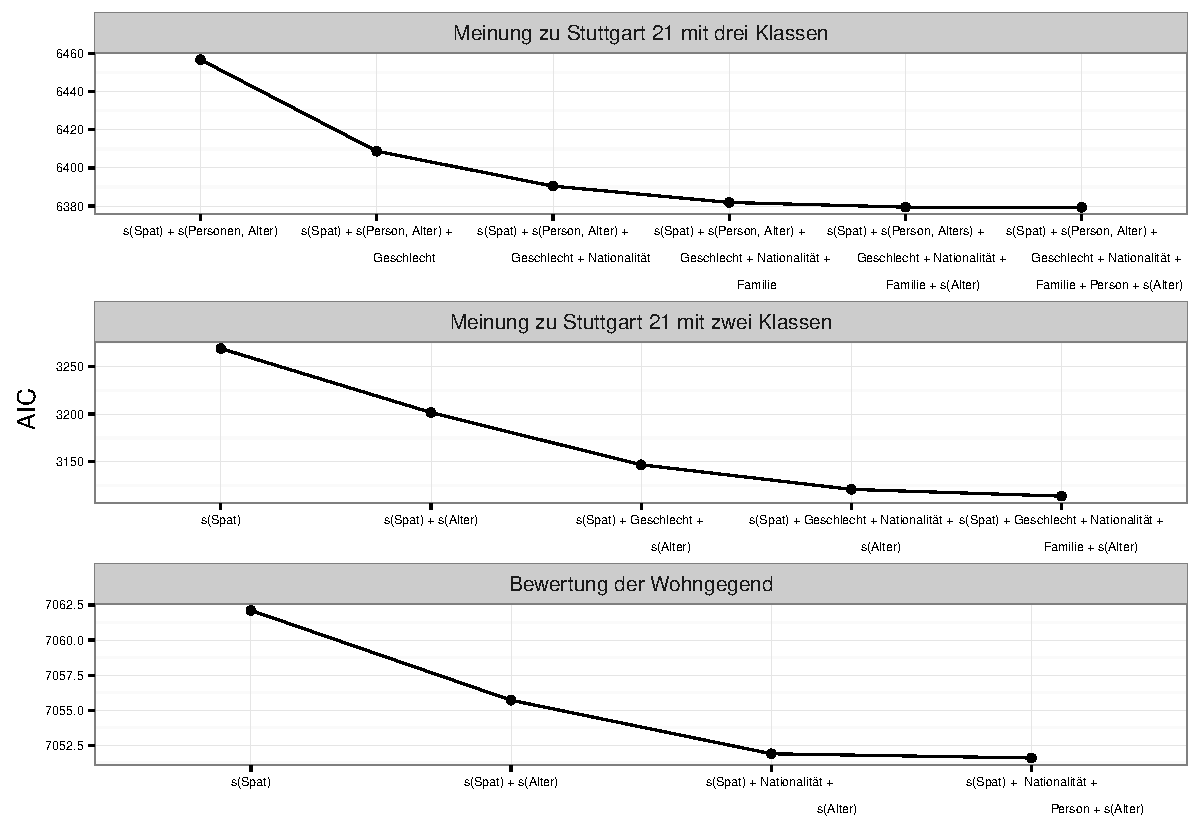
\includegraphics[scale=0.8]{Pictures/stepAIC}
 \caption{Konvergenz der äußeren Schleife der \textit{stepAIC} Funktion zur Ermittlung der optimalen Parameterkombinationen exemplarisch für alle Response Möglichkeiten mit Gauß-Krüger Informationen}
 \label{AIC}
 \end{center}
\end{figure}

Zu sehen ist, dass die Funktion für die Bewertung der Wohngegend bereits nach vier äußeren Iterationen keine Verbesserung des AIC mehr erreichen kann und die optimale Modellkomplexität gefunden wurde. Für die Modelle zur Meinung zu Stuttgart 21 ist die optimale Modellkomplexität nach fünf bzw. sechs äußeren Iterationen gefunden. Damit weist das drei Klassenmodell zur Meinung zu Stuttgart 21 die höchste Modellkomplexität auf. Ein interessantes Ergebnis der \textit{stepAIC} Funktion ist zudem, dass neben einer Hinzunahme der Wechselwirkung auch die Hinzunahme der Anzahl der im Haushalt lebenden Personen für das zwei Klassenmodell keine Verbesserung des AIC erreicht, obwohl beide Modelle im Prinzip das gleiche Problem behandeln. Die geringste Komplexität weißt das Modell zur Bewertung der Wohngegend auf. Es ist deutlich erkennbar, dass die Hinzunahme weiterer Kovariablen nach dem räumlichem Effekt nur eine sehr geringe Verbesserung des AIC bewirken, so ist die Differenz zwischen dem Modell nur mit räumlichem Effekt und dem bestem Modell nur ca 10 Punkte. Im Gegensatz dazu konnte durch die Hinzunahme von Kovariablen im zwei Klassenmodell zur Meinung zu Stauttgart 21 eine Verbesserung von ca 150 Punkten erreicht werden. Zu beachten ist jedoch auch, dass dies exemplarisch für die Gauss-Krüger Informationen ist und für die anderen räumlichen Effekte sind auch deutlich andere Parameterkombinationen anhand des AIC entstanden.
Insgesamt deutet das AIC für den drei Klassen Fall auf das Geoadditive Modell mit den Gauß-Krüger Informationen als qualitativ höchstes Modell hin. Beim zwei Klassen Fall schneidet das Geoadditive Modell in jedem Fall am besten ab, wobei hier das Modell mit Stadtteilen als räumlichem Effekt die höchste Qualität laut dem AIC aufweist.


\subsection{Modelle}
In Tabelle \ref{stepAIC} wird der Effekt der räumlichen Komponente auf die Modelle betrachtet. Über die schrittweise AIC Analyse wurde die geeignetste Kombination der sozioökonomischen Variablen festgelegt. Es ist zu beachten, dass die geeignete Kovariablenkombination mit den geoadditiven Modell einzeln ermittelt wurde. Um die Einflüsse der räumlichen Effekte isoliert bewerten zu können, blieb die zuvor ermittelte Kovariablenkombination innerhalb eines Modells gleich. Nach der Eliminierung des räumlichen Trends wurde also keine erneute AIC-basierende Kovariablenwahl durchgeführt. Die Kombination der sozioökonomischen Kovariablen ist in Tabelle \ref{stepAIC} folglich in jeder Zeile gleich. Die Kovariablenkombinationen der Modelle ohne räumlichen Effekt kann sich folglich unterscheiden. Jedes geoadditive Modell wird mit einem Modell ohne räumlichen Effekt sowie einem Modell nur mit dem räumlichen Effekt verglichen. Beim Vergleich muss beachtet werden, dass die AIC der Modelle nur als Indiz und nicht als hinreichendes Kriterium allein zur Modellwahl gelten können, da die Stichprobenumfänge nicht gleich sind. Zum einen wurden für die Modellierung auf Stadtbezirksebene Pseudobeobachtungen erstellt, zum anderen wurden Beobachtungen mit der Ausprägung \textit{Neutral} für das Modell mit zweikategorialer Response-Variablen entfernt. Zudem besitzt das zweikategoriale Modell ohnehin ein geringere Komplexität durch die geringe Anzahl der möglichen Ausprägungen der endogenen Variable.

\begin{table}[h]
\centering
\caption{AIC der erstellten Modelle.}
\label{stepAIC}
\begin{tabular}{llccc}
\hline \hline
\multicolumn{5}{c}{Meinung zu Stuttgart 21}                                                                                                                                            \\ \hline
                          & \multicolumn{1}{l|}{}             & \multicolumn{1}{c|}{\multirow{2}{*}{Geoadditives Modell}} & \multicolumn{1}{c|}{Modell ohne}       & Modell nur mit    \\
                          & \multicolumn{1}{l|}{}             & \multicolumn{1}{c|}{}                                     & \multicolumn{1}{c|}{räumlichem Effekt} & räumlichem Effekt \\ \hline
\multirow{3}{*}{Drei Kl.} & \multicolumn{1}{l|}{Gauß-Krüger} & \multicolumn{1}{c|}{6379,345}                             & \multicolumn{1}{c|}{6378,220}          & 6525,747          \\
                          & \multicolumn{1}{l|}{Bezirke}      & \multicolumn{1}{c|}{6380.659}                             & \multicolumn{1}{c|}{6379,725}              & 6528,284          \\
                          & \multicolumn{1}{l|}{Stadtteile}   & \multicolumn{1}{c|}{6456,706}                               & \multicolumn{1}{c|}{6535,627}          & 6605,946          \\ \hline
\multirow{3}{*}{Zwei Kl.} & \multicolumn{1}{l|}{Gauß-Krüger} & \multicolumn{1}{c|}{3114,141}                             & \multicolumn{1}{c|}{3116,130}           & 3268,484          \\
                          & \multicolumn{1}{l|}{Bezirke}      & \multicolumn{1}{c|}{3115,858}                             & \multicolumn{1}{c|}{3116,130}           & 3271,325          \\
                          & \multicolumn{1}{l|}{Stadtteile}   & \multicolumn{1}{c|}{3149,607}                              & \multicolumn{1}{c|}{3180,433}          & 3298,017          \\ \hline
\multicolumn{5}{c}{Bewertung der Wohngegend}                                                                                                                                           \\ \hline
                          & \multicolumn{1}{l|}{}             & \multicolumn{1}{c|}{\multirow{2}{*}{Geoadditives Modell}} & \multicolumn{1}{c|}{Modell ohne}       & Modell nur mit    \\
                          & \multicolumn{1}{l|}{}             & \multicolumn{1}{c|}{}                                     & \multicolumn{1}{c|}{räumlichem Effekt} & räumlichem Effekt \\ \hline
                          & \multicolumn{1}{l|}{Gauß-Krüger} & \multicolumn{1}{c|}{7054,163}                             & \multicolumn{1}{c|}{7318,815}          & 7064,751          \\
                          & \multicolumn{1}{l|}{Bezirke}      & \multicolumn{1}{c|}{7175,601}                             & \multicolumn{1}{c|}{7318,815}          & 7197,003          \\
                          & \multicolumn{1}{l|}{Stadtteile}   & \multicolumn{1}{c|}{8252,374}                             & \multicolumn{1}{c|}{8567,358}          & 8750,801          \\ \hline \hline
\end{tabular}
\end{table}


Bei der Meinung zu Stuttgart 21 in drei sowie in zwei Kategorien lässt sich erkennen, dass die geoadditiven Modelle stets gleiche oder etwas bessere AIC zeigen als die Modelle ohne räumlichen Effekt. Die Modelle ohne sozioökonomische Kovariablen schneiden stets am schlechtesten ab. Im direkten Vergleich haben die sozioökonomischen Variablen also einen höheren Erklärungsgehalt als die räumlichen Effekte. Die räumlichen Effekte verringern die Modell AIC jedoch nicht. Sie haben demnach ebenfalls erklärenden Gehalt. Die Form des räumlichen Effektes hat eine untergeordnete Rolle. Es spielt im Hinblick auf die relative Modellqualität kaum eine Rolle, ob der räumliche Effekt kontinuierlich oder diskret auf Bezirksebene modelliert wird.\\
Bei der Bewertung der Wohngegend hingegen wirkt sich der räumliche Effekt sehr viel stärker auf die relative Modellqualität aus. Alle Modelle mit räumlichen Effekten zeigen stets die niedrigsten AIC. Der Vergleich der Modelle nur mit sozioökonomischen Variablen zu den Modellen ohne sozioökonomische Variablen offenbart, dass die räumlichen Effekt sogar wichtiger als die sozioökonomischen Kovariablen sind. Der Vergleich der räumlichen Effekte zeigt, dass das kontinuierliche geoadditive Modell gegenüber den diskreten Modellen vorteilhaft ist.\\
Zusammenfassend ist zu sagen, dass die geoadditiven Modelle tendenziell zumindest gleichwertig zu den GAM ohne räumlichen Effekt sind.

\begin{figure}[h]
 \begin{center}
 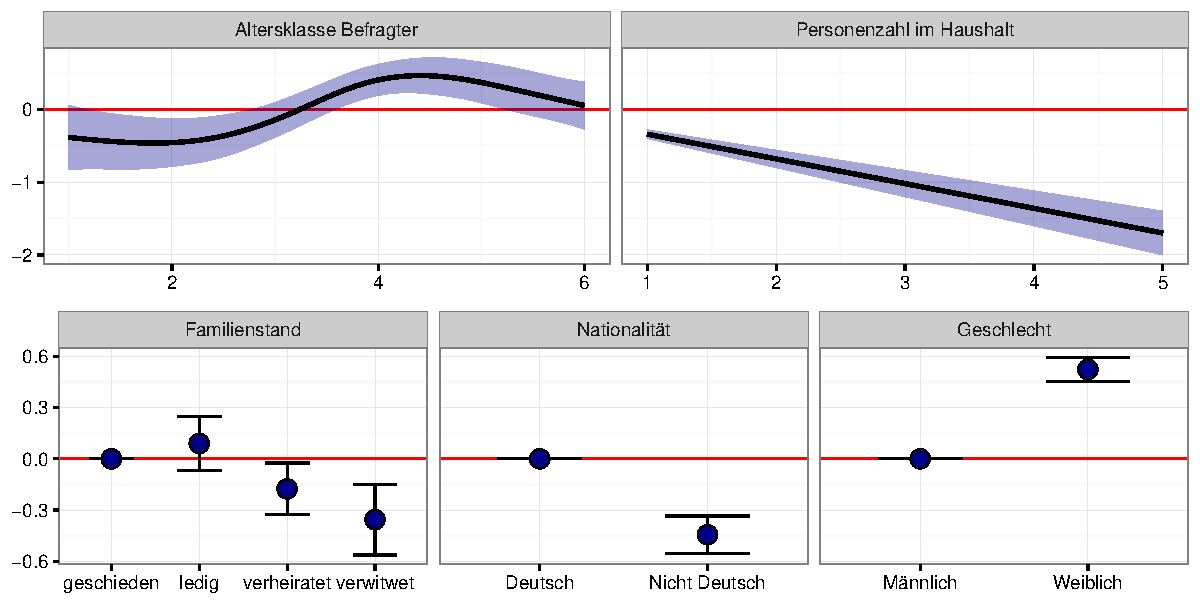
\includegraphics[scale=0.8]{Pictures/S21ModelEffects2}
 \caption{Univariate parametrische und nonparametrische Effekte des dreikategorialen Modells zur Vorhersage der Meinung zu Stuttgart 21 mit kontinuierlichem räumlichen Trend.}
 \label{GKParam}
 \end{center}
\end{figure}


\begin{figure}[htbp]
  \centering
 \subfigure[Kontinuierlich]{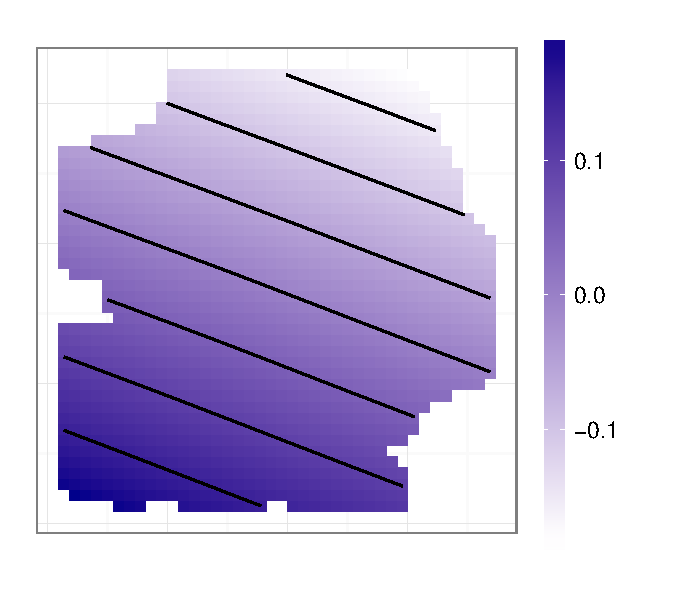
\includegraphics[scale=0.50]{Pictures/S21_3_Kont_SpatEff.pdf}}%\quad
  \subfigure[Diskret: Stadtbezirke]{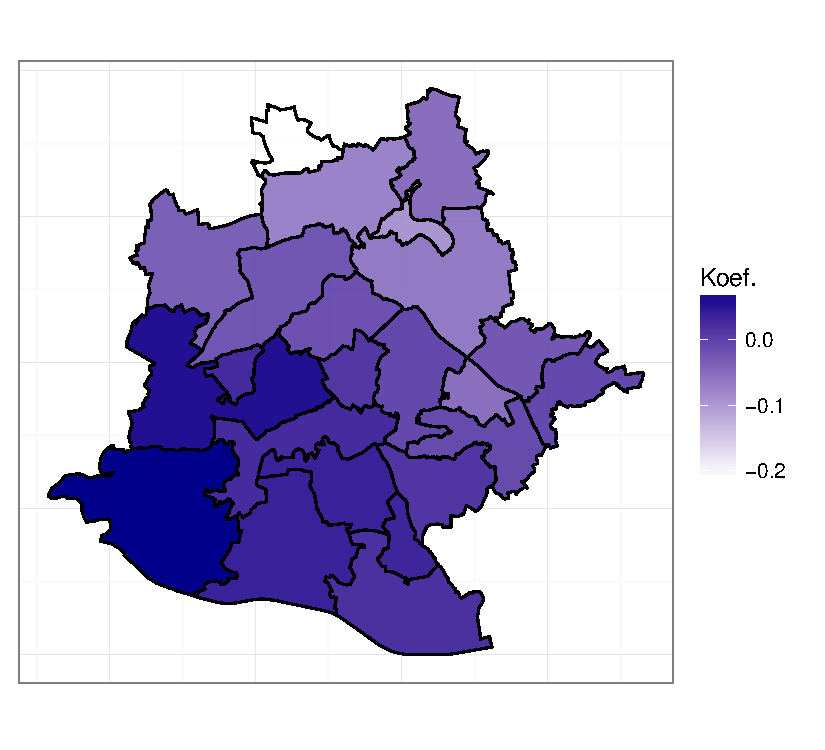
\includegraphics[scale=0.5]{Pictures/S21_3_Bezirke_SpatEff}}%\quad
  \subfigure[Diskret: Stadtteile]{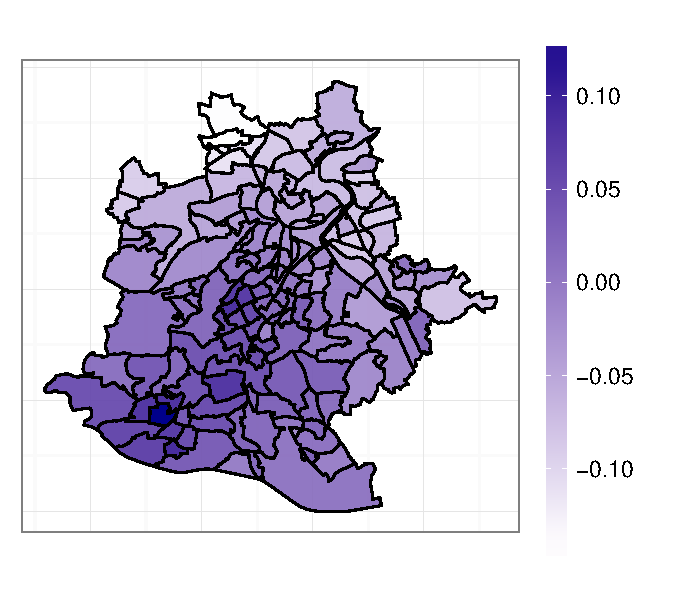
\includegraphics[scale=0.5]{Pictures/S21_3_Stadtt_SpatEff}}
  \caption{Räumliche Effekte des dreikategorialen Modells zur Vorhersage der Meinung zu Stuttgart 21.}
  \label{rEffS21}
\end{figure}

Der erste erstellte Modelltyp beschreibt die Meinung zu Stuttgart 21 in drei Kategorien (\textit{Zustimmung}, \textit{Neutral} und \textit{Ablehnung}) über die\textit{Altersklasse des Befragten}, die \textit{Personenzahl im Haushalt}, den \textit{Familienstand}, die \textit{Nationalität}, das \textit{Geschlecht} und den kontinuierlichem räumlichen Effekt. Aus Abbildung \ref{GKParam} und Tabelle \ref{ParameterTabS213spat} (A) geht die Signifikanz der Modellparameter hervor. Hierbei ist zu beachten, dass \textit{Zustimmung} mit 1 und \textit{Ablehnung} mit 3 kodiert wurde. Je höher der Effekt, desto höher ist also die Wahrscheinlichkeit der \textit{Ablehnung}. Die \textit{Altersklasse des Befragten} zeigte einen stark nichtlinearen Trend. Die Wahrscheinlichkeit der Ablehnung ist in den jüngeren Altersklassen bis 2 (15 bis 35 Jahre) am geringsten. Sie steigt bis zu ihrem Höhepunkt bei Altersklasse  4 und 5 (45 bis 65 Jahre) an und fällt dann relativ stark wieder ab. Die Personenzahl im Haushalt ging, entgegen der Erwartungen, parametrisch in das Modell ein. Der Effekt zeigt einen stark negativen linearen Trend. Die Wahrscheinlichkeit der \textit{Ablehnung} ist also in Single-Haushalten mit deutlichem Abstand am höchsten. Die Kategorien des Familienstands unterscheiden sich zwar nicht signifikant von 0, werden jedoch aufgrund der leichten AIC Verringerung berücksichtigt. Es ist ersichtlich, dass \textit{geschiedene} und \textit{ledige} Bürger eher eine ablehnende Haltung gegenüber Stuttgart 21 zeigen \textit{verheiratete} oder \textit{verwitwete}. Deutlicher sind die Effekte der Nationalität und des Geschlechts. \textit{Deutsche} Bürger zeigen eine signifikant höhere Ablehnungswahrscheinlichkeit als ausländische Bürger. Der Unterschied zwischen den Geschlechtern ist etwa ebenso stark. Männer haben eine geringere Ablehnungswahrscheinlichkeit als Frauen. Die beschriebenen Ausprägungen der sozioökonomischen Kovariablen finden sich in näherungsweise gleicher Ausprägung in allen dreikategorialen geoadditiven Vorhersagemodellen der Meinung zu Stuttgart 21 (Tabelle \ref{ParameterTabS213spat}). Ausnahme bildet einzig der Familienstand im diskreten räumlichen Modell auf Stadtbezirksebene, welcher nach schrittweiser AIC Analyse nicht in dieses Modell eingeflossen ist. Aus diesem Grunde stehen die Kovariablenausrprägungen stellvertretend für alle drei geoadditiven Modelle für die Vorhersage der Meinung zu Stuttgart 21 in drei Kategorien.\\
Die visuelle Überprüfung der unterschiedlichen Parameterausprägungen der räumlichen Effekte (Abbildung \ref{rEffS21}) offenbart ein deutliches Nord-Süd Gefälle der Ablehnungswahrscheinlichkeit. In \textit{Stammheim} im äußersten Norden ist der räumliche Einfluss auf den Prädiktor bei allen drei räumlichen Modellen unter -0,1 und damit am geringsten in ganz Stuttgart. Des weiteren ist die Ablehnungswahrscheinlichkeit in den nördlichen Bezirken \textit{Zuffenhausen}, \textit{Münster} und \textit{Bad Cannstadt} im Vergleich zu allen Stadtteilen sehr gering. Die Ablehnungswahrscheinlichkeit steigt tendenziell in südlicher Richtung. Etwa in der Mitte der Stadt, verlaufend vom Stadtbezirk \textit{Weilimsdorf} im Westen über \textit{Feuerbach}, \textit{Mitte} und \textit{Wangen} bis nach \textit{Obertürkheim} im Osten, ist der räumliche Modelleinfluss nahe 0. Südlich dieser Linie steigen die Parameterausprägungen tendenziell in südwestlicher Richtung. Im Bezirk \textit{Vaihingen} sind mit deutlichem Abstand die höchste Ablehnungswahrscheinlichkeiten zu sehen. Dieser grundsätzliche Trend ist in allen drei Modellen ähnlich ausgeprägt. Nach Stadtteilen aufgelöst (Abbildung \ref{rEffS21} (c)) lassen sich die räumlichen Trends jedoch noch kleinräumiger darstellen. Innerhalb des südlichen Bereichs (in dem die Ablehnung tendenziell höher ist) sind in dieser Auflösungsebene Hot-Spots sichtbar. So zeigt sich, dass die Ablehnungswahrscheinlichkeit innerhalb \textit{Vaihingens} inhomogen verteilt ist. Der Stadtteil \textit{Vaihingen-Mitte} zeigt die höchste Parameterausprägung aller Stuttgarter Stadtteile. Die Parameter der anderen Stadtteile \textit{Vaihingens} sind deutlich kleiner. Aus diesem Grunde ist die Skala der Parameterausprägung auf Stadtteilebene (Abbildung \ref{rEffS21} (c)) höher als auf Stadtbezirksebene Abbildung \ref{rEffS21} (b)). Weitere nennenswerte Abweichungen der Stadtteile innerhalb ihrer Bezirke ergeben sich nur noch in dem relativ großen Bezirk \textit{West}. Während die Haltung in \textit{Solitude} eher \textit{zustimmend} ist, nehmen Bürger aus \textit{Kräherwald} und \textit{Wildpark} eher eine Ablehnende Haltung ein. Dieser Stadtbezirk nimmt eine Sonderstellung ein, da er sehr wenige, in den Stadtteilen \textit{Kräherwald} und \textit{Wildpark} gar keine, Beobachtungen zeigt. Die Parameterausprägung ist demnach stark von den Nachbarregionen getrieben. In allen anderen Stadtbezirken Stuttgarts ist die Parameterausprägung innerhalb der Stadtteile vergleichsweise homogen. Hier entsprechen die Parameterausprägungen der Stadtteile folglich näherungsweise den Parameterausprägungen der dazugehörigen Stadtbezirke.\\
Die Effekte des zweiten Modelltyps, also des Vorhersagemodells mit zweikategorialer Response, sind praktisch gleich \ref{ParameterTabS212spat} zu dem Modell mit drei Kategorien. Auch hier ist ein Nord-Süd Gefälle ersichtlich. Der Bezirk \textit{Vaihingen} zeigt, insbesondere im Stadtteil \textit{Vaihingen-Mitte}, die höchste Ablehnungswahrscheinlichkeit, während diese in \textit{Stammheim} am geringsten ist.\\
\begin{figure}[h]
 \begin{center}
 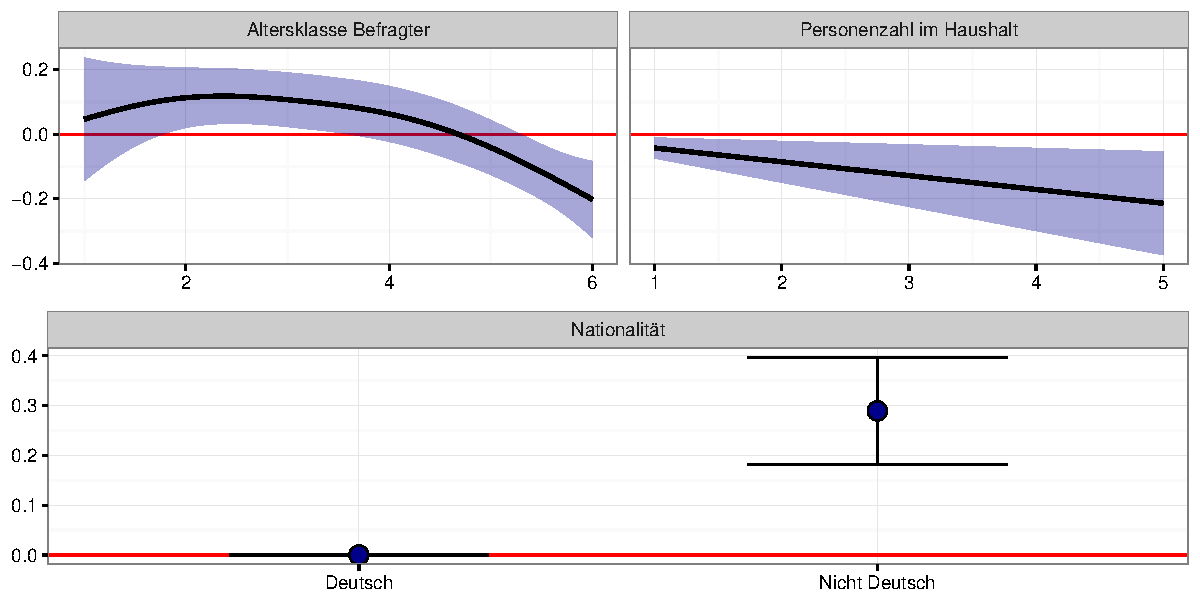
\includegraphics[scale=0.8]{Pictures/BWModelEffects2}
 \caption{Univariate parametrische und nonparametrische Effekte des Modells zur Vorhersage der Wohnzufriedenheit mit kontinuierlichem räumlichen Trend.}
 \label{BWParam}
 \end{center}
\end{figure}
Der dritte Modelltyp beschreibt die Wohnzufriedenheit in 5 Kategorien. Wobei \textit{sehr gut} mit 1 und \textit{sehr schlecht} mit 5 kodiert wurde. Je höher der Koeffizient des Prädiktors ausgeprägt ist, desto höher ist also die Wahrscheinlichkeit der unzufriedenen Kategorie anzugehören. Abbildung \ref{BWParam} und Tabelle \ref{ParameterTabW5spat} (A) zeigen die Zusammenfassung der sozioökonomischen Parameter des Modells mit kontinuierlichem räumlichen Effekt. Die \textit{Altersklasse des Befragten} geht als Spline in das Modell ein. Die Parameterausprägung stagniert zunächst bei etwa 0,08 bis 0,1 bis zu Altersklasse 4 (15 bis 55 Jahre) und sinkt dann relativ stark bis auf -0,2 ab. Die \textit{Peronenzahl im Haushalt} geht linear in das Modell ein. Die Wohnzufriedenheit sinkt stetig mit der Anzahl der Mitbewohner. Bei Single-Haushalten ist der Einfluss der Personenzahl nahe null. Am stärksten von allen sozioökonomischen Variablen wirkt sich die Nationalität auf die Wohnzufriedenheit aus. \textit{Nicht deutsche} Bürger Bewerten ihre Wohnsituation signifikant schlechter. Diese  sozioökonomischen Größen sind im geoadditiven Modell auf Stadtbezirksebene in gleicher Ausprägung zu finden (Tabelle \ref{ParameterTabW5spat} (B)). Beim Modell auf Stadtteilebene zeigte eine andere Kovariablenkombination den geringsten AIC (Tabelle \ref{ParameterTabW5spat} (C)).\\
Dem räumlichen Effekt kommt bei der Bewertung der Wohnzufriedenheit eine besondere Bedeutung zu. Wie anhand der absoluten Höhe der Parameterausprägung ersichtlich, hat der räumliche Effekt stärkeren Einfluss auf die Wohnzufriedenheit als die anderen Kovariablen. Der räumliche Effekt zeigt sich deutlich strukturierter als es bei der Meinung zu Stuttgart 21 der Fall war. Es sind kaum generelle Trends zu erkennen. Vielmehr unterscheidet sich die Wohnzufriedenheit relativ kleinräumig. Die geringsten Koeffizientenausprägungen, also die höchsten Wohnzufriedenheiten, des kontinuierlichen räumlichen Trends verlaufen in etwa vom Stadtviertel \textit{Feuerbacher Tal} in Richtung Südwest über \textit{Pfaffenwald} und \textit{Sternhäule} bis \textit{Sillenbruch} (Abbildung \ref{rEffW} (a)). Ausgehend von diesem relativ großen Bereich mit hoher Wohnzufriedenheit steigen die Koeffizienten in alle Richtungen an. Obwohl dieser Bereich der hohen Zufriedenheit sich relativ weit bis in den Süden erstreckt, steigen die Koeffizienten in südlicher Richtung, also in Richtung der Stadtteile \textit{Rohr}, \textit{Mohringen-Süd} und \textit{Plieningen}, bis zum Stadtrand nochmal deutlich an. Die Koeffizienten steigen, von dem Bereich mit hoher Wohnzufriedenheit ausgehend, in nordwestlicher Richtung ebenfalls abrupt an. Die höchsten  Koeffizienten sind etwa im Bereich der Bezirke \textit{Ost} und \textit{Wangen} zu beobachteten. Weiter östlich von dieser Region mit höchster Unzufriedenheit zeigen sich wieder sehr kleine Koeffizientenausprägungen. Der einzige Bereich mit vergleichsweise homogenen Parameterausprägungen ist der Nordosten Stuttgarts. In diesem Bereich nehmen die Koeffizienten Werte um null an. Die insgesamt sehr differenzierte räumliche Koeffizientenverteilung kann mit den Modellen auf Stadtteil-Basis nicht widergespiegelt werden, da die Auflösung zu gering ist (Abbildung \ref{rEffW} (b)). Durch die homogen hohe Wohnzufriedenheit ist der Koeffizient des Bezirks \textit{Degerloch} zwar mit deutlichem Abstand am kleinsten. In den anderen Bezirken des Südens zeigen die Parameterausprägungen jedoch nur relativ geringe negative Ausprägungen. Dies ist auf die inhomogene Wohnzufriedenheit innerhalb der Bezirke zurückzuführen. Die Wohnzufriedenheit zeigt innerhalb der drei großen Stadtbezirke des Südens ein starkes Nord-Süd-Gefälle. Eben dies gilt unter anderem für die Bezirke \textit{Bad Cannstadt}, \textit{Unter-} und \textit{Obertürkheim} im Westens. Im Nordwesten Stuttgarts zeigen sich, wie beim kontinuierlichen räumlichen Modell, Ausprägungen um null. Auf Ebene der Stadtteile zeigt sich entsprechend ein sehr diffiziles räumliches Muster (Abbildung \ref{rEffW} (c)). Die räumliche Verteilung der Parameterausprägungen ist mit den Parametern des kontinuierlichen Modells vergleichbar.

\begin{figure}[htbp]
  \centering
 \subfigure[Kontinuierlich]{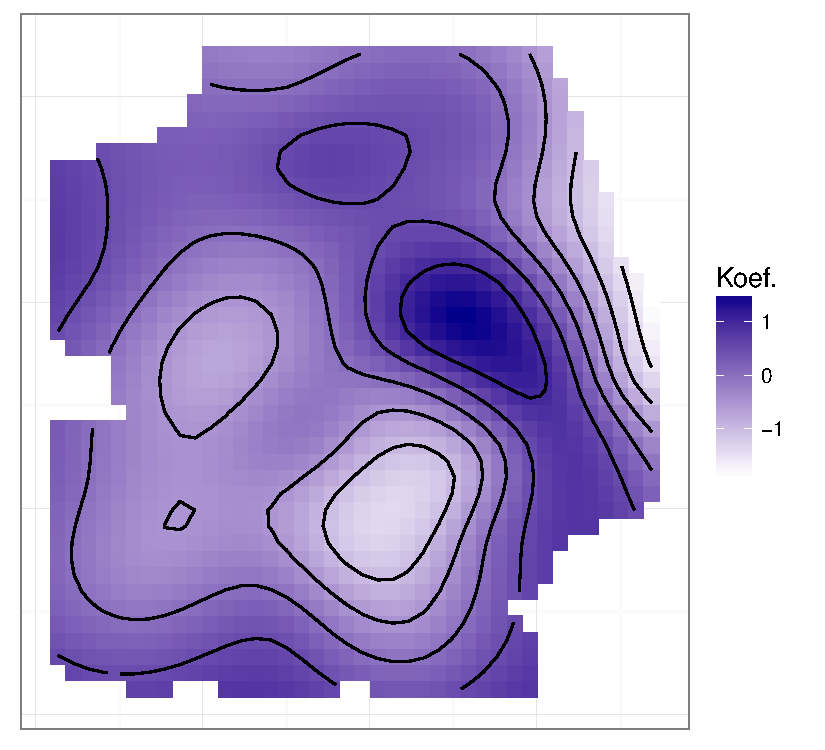
\includegraphics[scale=0.5]{Pictures/W_5_Kont_SpatEff.pdf}}%\quad
  \subfigure[Diskret: Stadtbezirke]{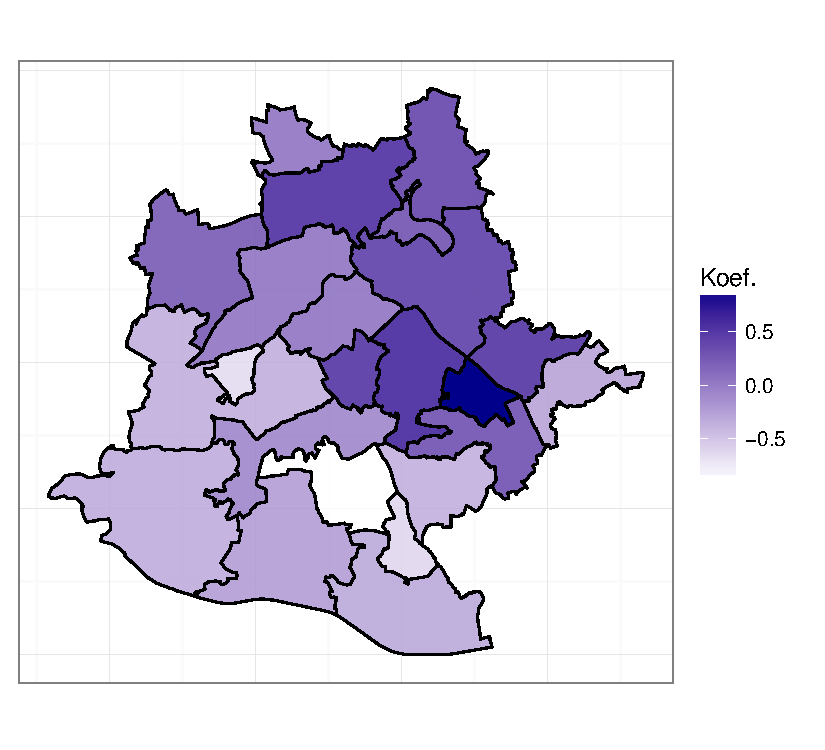
\includegraphics[scale=0.5]{Pictures/W_5_Bezirke_SpatEff}}%\quad
  \subfigure[Diskret: Stadtteile]{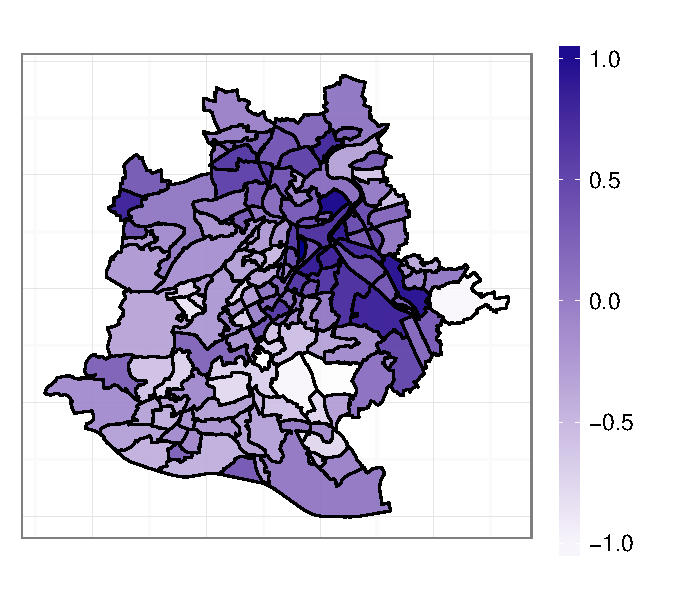
\includegraphics[scale=0.5]{Pictures/W_5_Stadtt_SpatEff}}
  \caption{Räumliche Effekte des Modells zur Vorhersage der Wohnzufriedenheit.}
  \label{rEffW}
\end{figure}

\subsection{Reklassifizierung}

Die Ergebnisse der Reklassifizierung zur Meinung zu Stuttgart 21 (Tabelle \ref{evalS21}) zeigen, dass die Erfolgsquote im drei Klassenmodell zwischen 44\% und 50\% liegt und im zwei Klassenmodell zwischen 55\% und 62\% liegt. Zum Vergleich mit einem reinen Zufallsmodell, dass im drei Klassenmodell eine Erfolgswahrscheinlichkeit von 1/3 und im zwei Klassenmodell von 1/2 hat, weisen die geschätzten Modelle eine höhere Erfolgsquote auf. Auch bei einem Vergleich mit Tabelle \ref{endogene} zeigt sich, dass die geschätzten Modelle besser abschneiden, als ein triviales Wählen der immer gleichen Klasse mit der höchsten Anzahl der Beobachtungen.

\begin{table}[h]
\centering
\caption{Mittlerer Anteil der korrekt reklassifizierten Beobachtungen zur Meinung zu Stuttgart 21.}
\label{evalS21}
\begin{tabular}{ll|c|c|c}
\hline \hline
                          &              & \multirow{2}{*}{Geoadditives Modell} & Modell ohne       & Modell nur mit    \\
                          &              &                                      & räumlichem Effekt & räumlichem Effekt \\ \hline
\multirow{3}{*}{Drei Kl.} & Gauß-Krüger & 0,4918                               & 0,4716            & 0,4732            \\
                          & Bezirke      & 0,4726                               & 0,4719            & 0,4726            \\
                          & Stadtteile   & 0,451                                & 0,4685            & 0,4449            \\ \hline
\multirow{3}{*}{Zwei Kl.} & Gauß-Krüger & 0,6193                               & 0,6104            & 0,5524            \\
                          & Bezirke      & 0,6079                               & 0,6104            & 0,5515            \\
                          & Stadtteile   & 0,6282                               & 0,6052            & 0,6099            \\ \hline \hline
\end{tabular}
\end{table}

Des weiteren ist zu sehen, dass das geoadditive Modell in fast allen Fällen die höchste Erfolgsquote aufweist. Abweichungen bestehen im drei Klassenmodell mit Stadtteilen als räumlichem Effekt und im zwei Klassenmodell mit Bezirken als räumlichem Effekt. Außerdem ist zu beachten, dass im drei Klassenmodell das Modell nur mit räumlichem Effekt besser abschneidet als das Modell ohne räumlichem Effekt, während sich für zwei Klassen diese Situation umgekehrt hat.\\
Für die Reklassifikation der Bewertung der Wohngegend (Tabelle \ref{evalB}) ergibt sich eine Erfolgsquote zwischen 40\% und 50\%. Damit ist auch hier eine deutliche Verbesserung gegenüber rein zufälligem Wählen oder dauerhaftem Wählen einer Klasse gegeben. 

\begin{table}[h]
\centering
\caption{Mittlerer Anteil der korrekt reklassifizierten Beobachtungen zur Bewertung der Wohngegend.}
\label{evalB}
\begin{tabular}{l|c|c|c}
\hline \hline
             & \multirow{2}{*}{Geoadditives Modell} & Modell ohne       & Modell nur mit    \\
             &                                      & räumlichem Effekt & räumlichem Effekt \\ \hline
Gauß-Krüger & 0,4922                               & 0,4461            & 0,4896            \\
Bezirke      & 0,4701                               & 0,4461            & 0,4621            \\
Stadtteile   & 0,4046                               & 0,4204            & 0,4347            \\ \hline \hline
\end{tabular}
\end{table}

Für die Modelle mit den kontinuierlichen Gauß-Krüger Informationen und den Bezirken als räumlichem Effekt hat das Geoadditive Modell die höchste Erfolgsrate, wohingegen für die Stadtteilinformationen das Modell nur mit räumlichem Effekt die beste Reklassifizierung aufweist. Insgesamt schneidet das Geoadditive Modell für beide endogene Variablen und alle drei möglichen Klassenanzahlen am besten ab. Außer bei dem zwei Klassenmodell zur Meinung zu Stuttgart 21 weisen beim Geoadditivem Modell die Stadtbezirke als räumliche Effekte die höchste und die Stadtteile als räumliche Effekte die niedrigste Erfolgsrate auf. Da die Modelle ohne- oder nur mit räumlichem Effekt in der AIC-Untersuchung und Reklassifizierung in den meisten Fällen schlechter Abschnitten, wurden die Ansätze ohne- oder nur mit räumlichem Effekte nicht weiter verfolgt und als beste Modelle zur Extrapolation ausgeschlossen.

\subsection{Kreuzvalidierung}

Die Kreuzvalidierung wurde vorgenommen, um die Vorhersagequalität außerhalb der eigenen Stichprobe der Modelle einzuschätzen. Die Ergebnisse zur Meinung zu Stuttgart 21 (Tabelle \ref{KreuzM}) zeigen eine ähnliche Erfolgsquote wie die innerhalb der Stichprobe vorgenommene Reklassifizierung (Tabelle \ref{evalS21}). Für das drei Klassenmodell liegt der Anteil der erfolgreich Klassifizierten Beobachtungen bei ca. 49\% und im zwei Klassenmodell zwischen 60\% und 63\%. Im drei Klassen Fall kann das Modell mit Stadtteilen als räumlichem Effekt ca. 3,5\%  mehr Beobachtungen richtig zuweisen als in der Reklassifizierung und das Modell mit Bezirken als räumlichem Effekt ca. 2\% mehr, womit es insgesamt auch die höchste Erfolgsrate aufweist. Die Erfolgsquote mit den Gauß-Krüger Informationen ist in etwa gleich geblieben, ähnlich wie die Modelle im zwei Klassen Fall.
 
\begin{table}[h]
\centering
\caption{Mittlerer Anteil korrekt klassifizierter Beobachtungen durch Kreuzvalidierung des Modells zu Modellierung der Meinung zu Stuttgart 21 nach einzelnen Klassen.}
\label{KreuzM}
\begin{tabular}{lcccccccccc}
\hline \hline
\multicolumn{11}{c}{Drei Klassen}                                                                                                                                                                                                        \\ \hline 
\multicolumn{1}{c}{}                                                     & \multicolumn{1}{c|}{}  & \multicolumn{3}{c|}{Gauß-Krüger}            & \multicolumn{3}{c|}{Bezirke}                 & \multicolumn{3}{c}{Stadtteile}         \\ \cline{3-11} 
                                                                         & \multicolumn{1}{c|}{}  & \multicolumn{9}{c}{Geschätzte Klasse}                                                                                                \\
                                                                         & \multicolumn{1}{c|}{}  & 1       & 2   & \multicolumn{1}{c|}{3}       & 1       & 2   & \multicolumn{1}{c|}{3}       & 1           & 2           & 3          \\ \hline
\multirow{3}{*}{\begin{tabular}[c]{@{}l@{}}Wahre \\ Klasse \end{tabular}} & \multicolumn{1}{c|}{1} & 0,756   & 0   & \multicolumn{1}{c|}{0,244}   & 0,754   & 0   & \multicolumn{1}{c|}{0,246}   & 0,746           & 0           & 0,254        \\
                                                                         & \multicolumn{1}{c|}{2} & 0,673   & 0   & \multicolumn{1}{c|}{0,327}   & 0,670   & 0   & \multicolumn{1}{c|}{0,330}   & 0,663          & 0           & 0,337        \\
                                                                         & \multicolumn{1}{c|}{3} & 0,521   & 0   & \multicolumn{1}{c|}{0,479}   & 0,511   & 0   & \multicolumn{1}{c|}{0,489}   & 0,509      & 0           & 0,491     \\ \hline
\multicolumn{2}{l|}{Klassifikation Modell}                                                        & \multicolumn{3}{c|}{\multirow{2}{*}{0,4905}} & \multicolumn{3}{c|}{\multirow{2}{*}{0,4928}} & \multicolumn{3}{c}{\multirow{2}{*}{0,4893}} \\
\multicolumn{2}{l|}{Insgesamt}                                                                    & \multicolumn{3}{c|}{}                        & \multicolumn{3}{c|}{}                        & \multicolumn{3}{c}{}                   \\ \hline
\multicolumn{11}{c}{Zwei Klassen}                                                                                                                                                                                                        \\ \hline
                                                                         & \multicolumn{1}{l|}{}  & \multicolumn{3}{c|}{Gauß-Krüger}             & \multicolumn{3}{c|}{Bezirke}                  & \multicolumn{3}{c}{Stadtteile}         \\ \cline{3-11} 
                                                                         & \multicolumn{1}{l|}{}  & \multicolumn{9}{c}{Geschätzte Klasse}                                                                                                \\
                                                                         & \multicolumn{1}{l|}{}  & 1       & \multicolumn{2}{c|}{2}             & 1       & \multicolumn{2}{c|}{2}             & 1           & \multicolumn{2}{c}{2}    \\ \hline
Wahre                                                                    & \multicolumn{1}{l|}{1} & 0,747   & \multicolumn{2}{c|}{0,253}         & 0,732   & \multicolumn{2}{c|}{0,268}         & 0,748         & \multicolumn{2}{c}{0,252}    \\
Klasse                                                                   & \multicolumn{1}{l|}{2} & 0,538   & \multicolumn{2}{c|}{0,462}         & 0,545   & \multicolumn{2}{c|}{0,455}         & 0,516       & \multicolumn{2}{c}{0,484}    \\ \hline
\multicolumn{2}{l|}{Klassifikation Modell}                                                        & \multicolumn{3}{c|}{\multirow{2}{*}{0,6193}} & \multicolumn{3}{c|}{\multirow{2}{*}{0,6079}} & \multicolumn{3}{c}{\multirow{2}{*}{0,6286}} \\
\multicolumn{2}{l|}{Insgesamt}                                                                    & \multicolumn{3}{c|}{}                        & \multicolumn{3}{c|}{}                        & \multicolumn{3}{c}{}                   \\ \hline \hline
\end{tabular}
\end{table}

Zudem lässt sich anhand von Tabelle \ref{KreuzM} die Trefferquote der einzelnen Klassen entnehmen. Die Tabelle zeigt die Anteile der Zuordnung von Beobachtungen der jeweiligen Klasse auf die eigene und jede der anderen Klassen. Die Hauptdiagonale liefert die Anteile der korrekt zugeordneten Beobachtungen. Die Einträge auf den Nebendiagonalen geben damit an, wie viele Beobachtungen einer Klasse relativ zur Gesamtzahl der Beobachtungen in eine falsche Klasse zugeordnet wurden. Markant ist, dass der zweiten Klasse in keinem Modell Beobachtungen zugeordnet wurden, weder falsch noch richtig. Mehrheitlich wurden diese der ersten Kategorie zugewiesen. Zudem ist die erste Klasse am öftesten richtig prognostiziert worden, allerdings wurden ihr auch die meisten falsch klassifizierten Beobachtungen zugeordnet. Dies gilt für alle drei Modelle. Im zwei Klassen Fall wurde das Problem der nicht geschätzten zweiten Klasse durch ihr auslassen umgangen. Allerdings findet sich auch hier ein deutlich häufigeres falsches zuordnen der zweiten Klasse in die erste als anders herum. 

\begin{table}[h]
\centering
\caption{Mittlerer Anteil korrekt klassifizierter Beobachtungen durch Kreuzvalidierung des Modells zu Modellierung Wohnzufriedenheit nach einzelnen Klassen.}
\label{KreuzBew}
\begin{tabular}{lc|ccccccccccccccc}
\hline \hline
\multicolumn{1}{c}{}                                                     &   & \multicolumn{5}{c|}{Gauß-Krüger}              & \multicolumn{5}{c|}{Bezirke}                   & \multicolumn{5}{c}{Stadtteile}              \\ \cline{3-17} 
                                                                         &   & \multicolumn{15}{c}{Geschätzte Klasse}                                                                                                        \\
                                                                         &   & 1     & 2     & 3 & 4 & \multicolumn{1}{c|}{5} & 1     & 2     & 3 & 4 & \multicolumn{1}{c|}{5} & 1       & 2       & 3       & 4   & 5       \\ \hline
\multirow{5}{*}{\begin{tabular}[c]{@{}l@{}}W. \\ Kl.\end{tabular}} & 1 & 0,445 & 0,555 & 0 & 0 & \multicolumn{1}{c|}{0} & 0,387 & 0,613 & 0 & 0 & \multicolumn{1}{c|}{0} & 0,495   & 0,478   & 0,019   & 0   & 0,008   \\
                                                                         & 2 & 0,254 & 0,746 & 0 & 0 & \multicolumn{1}{c|}{0} & 0,252 & 0,748 & 0 & 0 & \multicolumn{1}{c|}{0} & 0,300   & 0,671   & 0,023   & 0   & 0,006   \\
                                                                         & 3 & 0,149 & 0,845 & 0 & 0 & \multicolumn{1}{c|}{0} & 0,153 & 0,847 & 0 & 0 & \multicolumn{1}{c|}{0} & 0,142   & 0,771   & 0,079   & 0   & 0,008   \\
                                                                         & 4 & 0,141 & 0,859 & 0 & 0 & \multicolumn{1}{c|}{0} & 0,141 & 0,859 & 0 & 0 & \multicolumn{1}{c|}{0} & 0,099   & 0,474   & 0,349   & 0   & 0,078   \\
                                                                         & 5 & 0,114 & 0,886 & 0 & 0 & \multicolumn{1}{c|}{0} & 0,086 & 0,914 & 0 & 0 & \multicolumn{1}{c|}{0} & 0,031   & 0,275   & 0,556   & 0   & 0,138   \\ \hline
\multicolumn{2}{l|}{Klass.}                                              & \multicolumn{5}{c|}{\multirow{3}{*}{0,4918}}   & \multicolumn{5}{c|}{\multirow{3}{*}{0,4704}}   & \multicolumn{5}{c}{\multirow{3}{*}{0,4594}} \\
\multicolumn{2}{l|}{M.}                                                  & \multicolumn{5}{c|}{}                          & \multicolumn{5}{c|}{}                          & \multicolumn{5}{c}{}                        \\
\multicolumn{2}{l|}{Insg.}                                               & \multicolumn{5}{c|}{}                          & \multicolumn{5}{c|}{}                          & \multicolumn{5}{c}{}                        \\ \hline  \hline
\end{tabular}
\end{table}

Tabelle \ref{KreuzBew} ist analog zu Tabelle \ref{KreuzM} aufgebaut. Das Ergebnis der Kreuzvalidierung für die Bewertung der Wohngegend ist, dass die Erfolgsquote zwischen ca. 46\% und 49\% liegt. Die Modelle mit Gauß-Krüger Informationen und Bezirken als räumlichen Effekten haben vergleichbar wie in der Reklassifizierung abgeschnitten. Das Modell mit den Stadtteilen hingegen weißt eine ca 5\% höhere Genauigkeit auf. Insgesamt jedoch behält das Modell mit den Gauß-Krüger Informationen die höchste Erfolgsrate. Auffällig ist auch hier, dass eine Klasse in keinem Modell Beobachtungen zugewiesen bekommen hat und zwei weitere Klassen in zwei von drei Modellen keine Beobachtungen zugewiesen bekommen haben. Abbildung \ref{endogene} gibt dabei einen Hinweis auf die Ursache dieses Phänomens, denn die Kategorien \textit{sehr gut} und \textit{gut} sind überproportional häufig im Datensatz vertreten im Vergleich zu den Klassen \textit{schlecht} und \textit{sehr schlecht}, weshalb schon durch die relative Häufigkeit die Wahrscheinlichkeit dass eine Beobachtungen in einer der letzten drei Kategorien ist, sehr klein wird. Bei der Bewertung der Wohngegend wurde am häufigsten die zweite Klasse sowohl richtig als auch falsch geschätzt.\\
Durch das relativ hohe Überschätzen einer Klasse bei beiden endogenen Variablen, sowie das totale Unterschätzen einiger Klassen, wird in der weiteren Validierung und Extrapolation auf das Vorhersagen einzelner Beobachtungen verzichtet. Stattdessen wird in einem bestimmten Gebiet über die Wahrscheinlichkeiten der Beobachtungen aggregiert und ein Anteil geschätzt, um auch geringere Wahrscheinlichkeiten für Beobachtungen zu berücksichtigen.

\subsection{Kleinräumige Extrapolation}
Bei der kleinräumigen Extrapolation ergab sich für die Modelle zur Modellierung der Meinung zu Stuttgart 21 die Möglichkeit der Validierung mit den Ergebnissen der Volksabstimmung. Daher werden die beiden geoadditiven Modelle (zwei- und dreikategorielle Response) vor der eigentlichen Darstellung der Extrapolation zunächst validiert.

\subsubsection{Validierung}
Die Ergebnisse der Validierung sind aus Tabelle \ref{vali} ersichtlich. Die Tabelle zeigt die MSE der prognostizierten Anteile aus den Modellen in Bezug auf die Anteile aus der Volksabstimmung. In der linken Spalte ist kodiert, welches der parametrisierten geoadditiven Modelle verwendet wurde und auf welche Datei diese Modelle zu Extrapolation angewendet wurden. Ganz links in dieser Spalte ist die Anzahl der Variablenausprägung der Response zu sehen. Daraufhin wird die Form des räumlichen Effekts beschrieben. Die nächste Angabe ist die Aggregationsebene auf der die kleinräumige Extrapolation durchgeführt wurde. Die letzte Angabe der ersten Spalte verschlüsselt den Namen der Datei mit der die Extrapolation durchgeführt wurde (\textit{M}: Melderegister, \textit{Z}: Zensus). Die mittlere Spalte zeigt die MSE für die beiden Kategorien der Volksabstimmung. Die rechte Spalte zeigt die Überdeckungswahrscheinlichkeit dieser beiden Kategorien. Demnach zeigt die erste Zeile beispielsweise die statistischen Gütemaße des geoadditiven Modells mit dreikategorieller Response und kontinuierlichem räumlichen Effekt aggregiert auf Bezirksebene mit den datensätzen des Melderegisters an. Die Prognoseintervalle zur Berechnung der Überdeckungswahrscheinlichkeit wurden über Bootstrap-Wiederholungen (siehe \textit{Statistische Methoden}) ermittelt.

\begin{table}[h]
\centering
\caption{Mittlere quadratische Abweichungen (MSE) und der Überdeckungs"-wahrscheinlichkeiten der Prognosen für die Meinung zu Stuttgart 21.}
\label{vali}
\begin{tabular}{llll|cc|cc}
\hline \hline
                        &                               &                          &   & \multicolumn{2}{c|}{MSE} & \multicolumn{2}{c}{Überdeckungswk.} \\
                        &                               &                          &   & Zustimmung  & Ablehnung  & Zustimmung        & Ablehnung       \\ \hline
\multirow{12}{*}{3 Kl.} & \multirow{4}{*}{Gauß-Krüger} & \multirow{2}{*}{Bez.}    & M & 0,04        & 0,749      & 1                 & 0,043           \\
                        &                               &                          & Z & 0,116       & 0,557      & 0,391             & 0               \\ \cline{3-8} 
                        &                               & \multirow{2}{*}{Sadtt.}  & M & 0,461       & 5,708      & 0,954             & 0,139           \\
                        &                               &                          & Z & 0,813       & 4,415      & 0,553             & 0,02            \\ \cline{2-8} 
                        & \multirow{4}{*}{Bezirke}      & \multirow{2}{*}{Bez.}    & M & 0,041       & 0,756      & 1                 & 0,043           \\
                        &                               &                          & Z & 0,117       & 0,562      & 0,522             & 0               \\ \cline{3-8} 
                        &                               & \multirow{2}{*}{Stadtt.} & M & 0,482       & 5,678      & 0,934             & 0,139           \\
                        &                               &                          & Z & 0,835       & 4,38       & 0,567             & 0,027           \\ \cline{2-8} 
                        & \multirow{4}{*}{Stadtteile}   & \multirow{2}{*}{Bez.}    & M & 0,032      & 0,862     &      1             &   0,043          \\
                        &                               &                          & Z & 0,148       & 0,552      &     0,478         &     0 \\ \cline{3-8} 
                        &                               & \multirow{2}{*}{Stadtt.} & M & 0,646       & 6,367       &   0,947           &   0,225  \\
                        &                               &                          & Z & 1,078        & 4,336       &   0,66           &                0,1 \\ \hline
\multirow{12}{*}{2 Kl.}  & \multirow{4}{*}{Gauß-Krüger} & \multirow{2}{*}{Bez.}   & M & 0,312      & 0,312      &     0,826           &  0,826
 \\
                        &                               &                          & Z & 0,152      & 0,152      &   0,522           &  0,522     \\ \cline{3-8} 
                        &                               & \multirow{2}{*}{Stadtt.} & M & 2,694       & 2,679     &   0,649          &  0,649   \\
                        &                               &                          & Z & 1,581       & 1,569      &  0,46            &   0,46   \\ \cline{2-8} 
                        & \multirow{4}{*}{Bezirke}      & \multirow{2}{*}{Bez.}    & M & 0,312       & 0,312      &  0,826            &   0,826    \\
                        &                               &                          & Z & 0,153       & 0,153      &  0,565            &  0,565    \\ \cline{3-8} 
                        &                               & \multirow{2}{*}{Stadtt.} & M & 2,642       & 2,645      &  0,636           &   0,636    \\
                        &                               &                          & Z & 1,527       & 1,513    &  0,433            &    0,44   
\\ \cline{2-8} 
                        & \multirow{4}{*}{Stadtteile}   & \multirow{2}{*}{Bez.}    & M & 0,524       & 0,524      &   0,043          &    0,043 \\
                        &                               &                          & Z & 0,172       & 0,172      &     0,652        &     0,652 \\ \cline{3-8} 
                        &                               & \multirow{2}{*}{Stadtt.} & M & 2,813        &  2,797      &  0,848     &  0,848 \\
                        &                               &                          & Z & 1,758        & 1,746     &    0,693     &     0,713
                         \\ \hline \hline
\end{tabular}
\end{table}

Zunächst wird das dreikategoriale geoadditive Modell mit dem zweikategorialen Modell verglichen .Bei der \textit{Ablehnung} zeigt sich, dass das zwei-Klassen-Modell stets kleinere MSE und höhere Überdeckungswahrscheinlichkeit annimmt. Es ist also zunächst besser als das Modell mit drei Kategorien. Das drei-Klassen-Modell überdeckt den wahren Wert nur sehr selten. Bei der \textit{Zustimmung} ergibt sich ein komplett konträres Ergebnis. Hier ist die mittlere quadratische Abweichung bei jeder Kombination im zwei-Klassen-Modell deutlich geringer als im drei Klassenmodell. Auch die Überdeckungswahrscheinlichkeit ist insbesondere bei den Ergebnissen zum Melderegister sehr viel höher. Zur Verdeutlichung dieser Ergebnisse zeigt Abbildung \ref{vali4} die Lage der geschätzten Anteile im Vergleich zu den wahren Anteilen für die \textit{Zustimmung}. Es ist zu erkennen, dass die prognostizierten Anteile des Drei-Klassen-Modells sehr nah an den wahren Anteilen liegen. Bemerkenswert ist, dass auf Bezirksebene der Anstieg der 45-Grad Linie sehr genau widergespiegelt wird. Die Prognosen sind also im gesamten Wertebereich sehr genau. Auf Stadtteilebene sind die extremen Werte (die es auf Bezirksebene nicht gibt) am Rand der Punktwolke schlechter getroffen. Beim Zwei-Klassen-Modell ist zu erkennen, dass die wahren Anteile sowohl auf Bezirks- als auch auf Stadtteilebene deutlich überschätzt werden. Des weiteren ist zu sehen, dass die Prognoseintervalle im zwei Klassenmodell eine starke Asymmetrie aufweisen, während die Prognoseintervalle des drei Klassenmodells symmetrisch sind.

\begin{figure}[h]
 \begin{center}
 
\includegraphics[scale=0.8]{Pictures/PaT2}
 \caption{Geschätzte gegen wahre prognostizierte Anteile der Zustimmung zu Stuttgart 21 der geoadditiven Modelle mir zweikategorialer und dreikategoriealer Response (je mit kontinuierlicher räumlicher Information). Zur Extrapolation wurde die Melderegister-Datei ausgewählt. Zusätzlich zu den Prognosen sind die 95\%-Quantile dargestellt.}
 \label{vali4}
 \end{center}
\end{figure}

Zusammenfassend kann gesagt werden, dass das geoadditive Modell mit dreikategorialer Response-Variable bei der Validierung besser abschneidet, da es die \textit{Zustimmung} sehr genauer bestimmen kann. Das Modell mit zweikategorialer Response wird deshalb für die kleinräumige Extrapolation nicht weiter verwendet. Innerhalb des Drei-Klassen-Modells lässt sich anhand von Tabelle \ref{vali} nicht eindeutig bestimmen, welcher räumliche Effekt der beste ist. Die größten Unterschiede, sowohl bei dem MSE als auch bei der Überdeckung, treten zwischen den Dateien auf.

\subsubsection{Pronose}
Die Modelle, die sich im Verlauf der Arbeit als vorteilhaft herausgestellt haben werden in diesem Unterkapitel an den Extrapolationsdateien angewendet. Hier werden also die eigentlichen Prognosen der Meinung zu Stuttgart 21 und der Wohnzufriedenheit Stuttgarts durchgeführt. Dazu zeigt Abbildung \ref{S21Alle} die extrapolierten Anteile der Modelle zur Meinung zu Stuttgart 21. Dargestellt ist der Median als Punktschätzung zusammen mit den Prognoseintervallen. Über die Zeilenbeschriftung wird die Prognostizierte Kategorie (1: \textit{Zustimmung}, 2: \textit{Neutral}, 3: \textit{Ablehnung}), der räumliche Trend des geoadditiven Modells für die Hochrechnung sowie die Extra\-polations\-datei (Z: \textit{Zensus}, M: \textit{Melderegister}) kodiert. Neben den kleinräumigen Extrapolationen zeigt Abbildung \ref{S21Alle} die Anteile, die sich ohne kleinräumige Extrapolation direkt aus der Parametrisierungsstichprobe als arithmetische Mittelwerteergeben ergeben hätten (gestrichelte Linie). Die Ergebnisse der Volksabstimmung sind zusätzlich als durchgezogene Linien dargestellt. Es zeigt sich eindeutig, dass sich die extrapolierten Anteile stark von den direkt aus den Rohdaten berechneten Anteilen unterscheiden. Während die \textit{neutrale} Kategorie vergleichbar ist, ist der geschätzte Anteil der \textit{Ablehnung} durch die kleinräumige Extrapolation deutlich gesunken, der Anteil der \textit{Zustimmung} folglich in gleichem Maße gestiegen. Es ist des weiteren erkennbar, dass sich die extrapolierten Anteile zwischen den Zensus und dem Melderegister teils deutlich unterscheiden. Die kleinräumige Extrapolation des Zensus prognostiziert eine \textit{Zustimmung} von ca. 47,1\%. Die kleinräumige Extrapolation der Daten des Melderegisters liegt sehr nah am Ergebnis der Volksabstimmung von 52,9\%. 

\begin{figure}[h]
 \begin{center}
 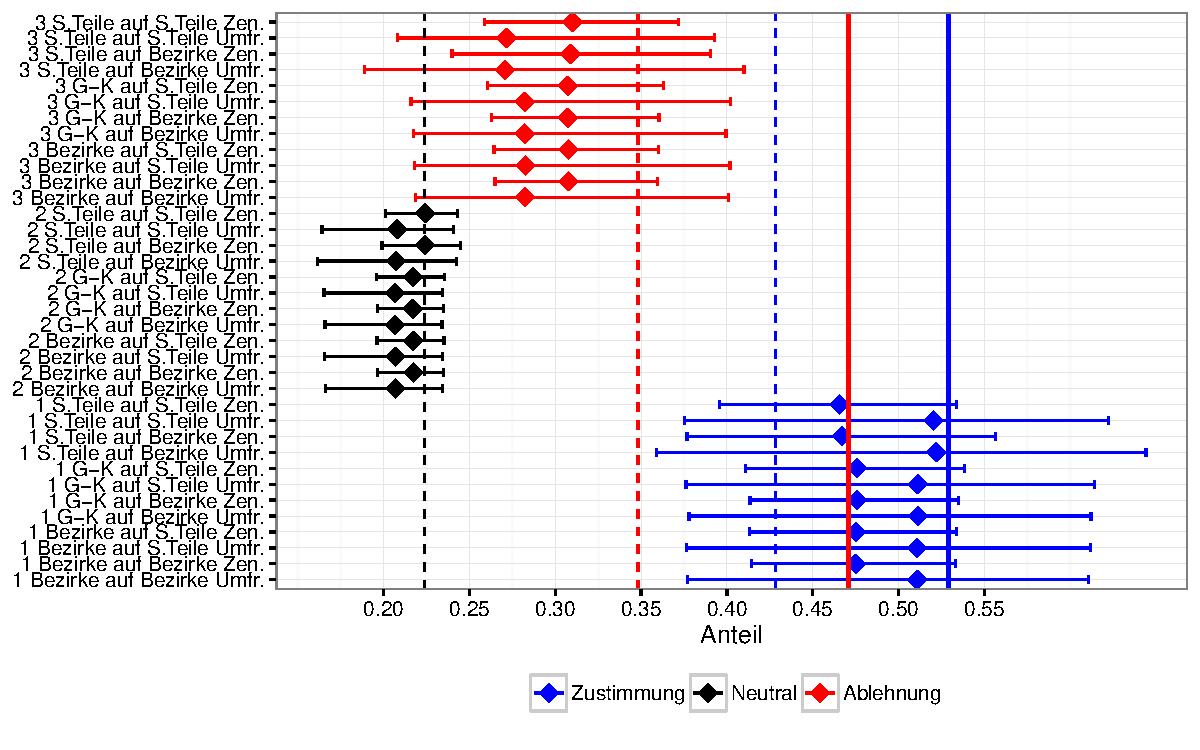
\includegraphics[scale=0.8]{Pictures/S21AlleModelle}
 \caption{Anteile der Meinung zu Stuttgart 21 nach kleinräumiger Extrapolation für ganz Stuttgart mit drei verschiedenen Schätzmodellen und zwei unterschiedlichen Datengrundlagen. Dargestellt sind die Punktschätzungen und die 95\% Quantile.}
 \label{S21Alle}
 \end{center}
\end{figure}

Durch kleinräumige Extrapolation mit dem Prognosemodell mit kontinuierlichem räumlichen Trend (\textit{Gauß-Krüger}) auf Basis der Melderegister Daten wurden 51,12\% \textit{Zustimmung} prognostiziert. Anwendung des Modells mit diskretem räumlichen auf Stadtbezirksebene (\textit{Bezirke}) ergab einen Anteil von 51,09\%, des Modells auf Stadtteilebene einen Anteil von 52,06\%. Die prognostizierten Anteile der \textit{neutrale} Klasse betragen 20,65\% bei Anwendung räumlich-kontinuierlichen Modells, 20,67\% beim diskreten räumlichen Modell auf Bezirks Ebene und 20,78\% beim diskreten räumlichen Modell auf Stadtteil Ebene. Für die Klasse \textit{Ablehnung} betragen die prognostizierten Anteile in gleicher Reihenfolge 28,22\%, 28,23\% und 27,15\%.\\
Die Extrapolationsergebnisse der geoadditiven Modelle mit kontinuierlichem räumlichen Effekt und der geoadditiven Modelle mit diskretem Effekt auf Stadtbezirksebene liegen stets nah beieinander. Das Ergebnis des Modells auf Stadtteilebene weicht in der Regle leicht von diesen beiden Ergebnissen ab. Auffällig sind die teils breiten Prognoseintervalle. Das Modell mit diskretem geoadditiven Term auf Stadtteilebene zeigt in der Regel die breitesten Intervalle.

\begin{figure}[h]
 \begin{center}
 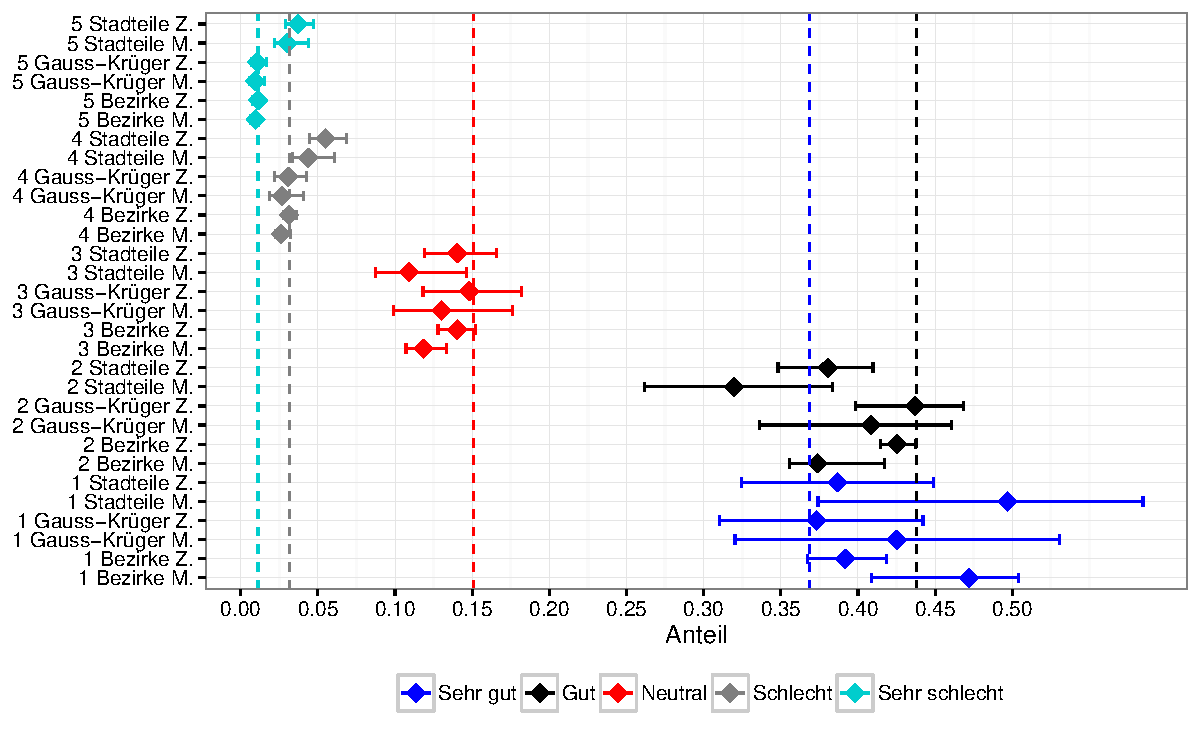
\includegraphics[scale=0.8]{Pictures/WohngegendAlleModelle2}
 \caption{Anteile der Bewertung der Wohngegend nach kleinräumiger Extrapolation für ganz Stuttgart mit drei verschiedenen Schätzmodellen und zwei unterschiedlichen Datengrundlagen. Dargestellt sind die Punktschätzungen und die 95\% Quantile.}
 \label{WAlle}
 \end{center}
\end{figure}

Die Ergebnisse der Extrapolation für die Bewertung der Wohngegend sind aus Abbildung \ref{WAlle} ersichtlich. Die Darstellung entspricht in ihrem Aufbau der Abbildung \ref{S21Alle}. Es ist auch hier zu sehen, dass die direkt per Mittelwert aus der Parametrisierungsstichprobe berechneten Anteile teils von den Anteilen nach der kleinräumigen Extrapolation abweichen. Bei den Klassen 3 (\textit{neutral}), 2 (\textit{gut}) und 1 (\textit{sehr gut}) ist ein deutlicher Unterschied erkennbar.
Teils werden die direkt berechneten Mittelwerte von den Prognoseintevallen der kleinräumigen Extrapolation nicht geschnitten. Es kann demnach durch visuelle Einschätzung von einem signifikanten Unterschied ausgegangen werden. Es zeigt sich auch bei der Modellierung der Wohnzufriedenheit, dass die Schätzung von den Extrapolationsdateien abhängt. Teilweise Unterscheiden sich die geschätzten Anteile beim \textit{Melderegister} und beim \textit{Zensus}. Die Ergebnisse auf Grundlage des \textit{Melderegisters} werden im folgenden der Übersichtlichkeit halber stellvertretend für alle Ergebnisse näher beschrieben. Aggregiert für gesamt Stuttgart ergeben sich für die Klasse \textit{sehr gut} 42,52\% für das Gauß-Krüger Modell, 47,18\% für das Bezirkmodell und 49,71 \% für das Stadtteilmodell. Für die Klasse \textit{gut} wurden 40,84\% für das Gauß-Krüger Modell, 37,37\% für das Bezirkmodell und 31,98 \% für das Stadtteilmodell prognostiziert. Die Klasse \textit{neutral} wurde von den Modellen in bisheriger Reihenfolge mit 13,08\%, 11,86\% und 10,91\% ermittelt. Die prognostizierten Anteile der Personen mit der Meinung \textit{schlecht}  sind 2,68\%, 2,61\% und 4,37\% . Die letzte Klasse \textit{sehr schlecht} wurde mit 0,95\%, 0,97\% und 3,03\% vorhergesagt. Im Vergleich zur Auswertung zur Meinung zum Projekt Stuttgart 21 hängen die Ergebnisse der Modllierung der Wohnzufriedenheit stärker vom gewählten Modell ab. Auch die Prognoseintervalle unterscheiden sich relativ stark zwischen den Modellen. Das Bezirke liefert in der Regel die schmalsten Prognoseintervalle.\\
Zuletzt wurden die beiden Modelle mit diskretem räumlichen Term genutzt um die Meinung zu Stuttgart 21 und die Wohnzufriedenheit auf Stadtteilebene zu prognostizieren. Für die Meinung zu Stuttgart 21 (Abbildung \ref{S21Extra}) kann dazu gut ein Vergleich mit den direkten Anteilen der Parametrisierungsstichprobe aus den Abbildungen \ref{XYStuttgart3}, \ref{BStuttgart21} und \ref{SStuttgart21} vorgenommen werden. Dabei zu beachten ist, dass Abbildung \ref{S21Extra} mit unterschiedlicher Skalierung dargestellt wird. Zunächst ist die räumliche Segregation mit erhöhtem Anteil der \textit{Zustimmung} im Norden, der \textit{neutralen} Haltung im Zentrum und \textit{Ablehnung} im Süden und Südwesten noch deutlich sichtbar.

\begin{figure}[h]
 \begin{center}
 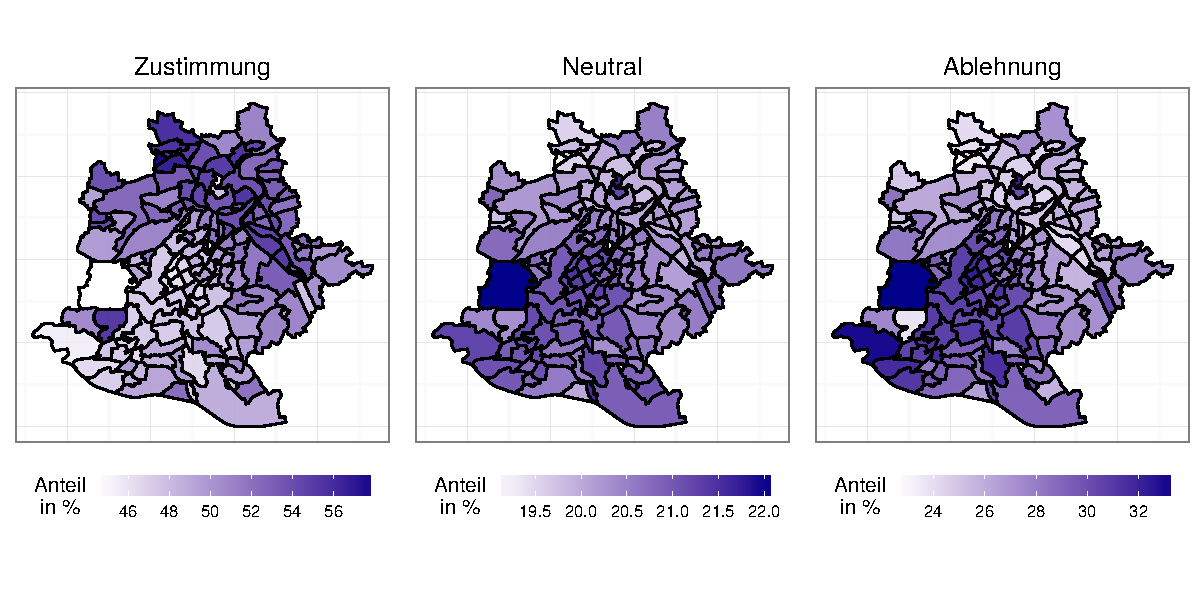
\includegraphics[scale=0.8]{Pictures/S21Extra}
 \caption{Extrapolierte Anteile auf Stadtteilebene für die Meinung zu Stuttgart 21 mit dem besten Modell.}
 \label{S21Extra}
 \end{center}
\end{figure}

Auch für die Bewertung der Wohngegend (Abbildung \ref{WohnExtra}) lässt sich ebenfalls ein Vergleich mit den Anteilen des Parametrisierungsdatensatzes (Abbildungen \ref{XYWohnG5}, \ref{BWohn} und \ref{SWohn}) vornehmen. Wie in den Rohdaten ist die räumliche Verteilung der Wohnzufriedenheit sehr kleinräumig strukturiert. Während die \textit{sehr guten} Einschätzungen vor allem südlich des Stadtzentrums zu finden sind, sind die \textit{guten} Bewertungen eher zentral bis nördlich lokalisiert. An den Stadträndern und sowie häufiger in Hot-Spots mitten zwischen den besseren Kategorien finden sich höhere Anteile der Kategorien \textit{schlecht} und \textit{sehr schlecht}. Besonders interessant ist, dass die schlechtesten Bewertungen in den Stadtvierteln \textit{Wasen} und \textit{Benzviertel} und den umliegendem Stadtteilen nördlich des Stadtzentrums liegen.

\begin{figure}[h]
 \begin{center}
 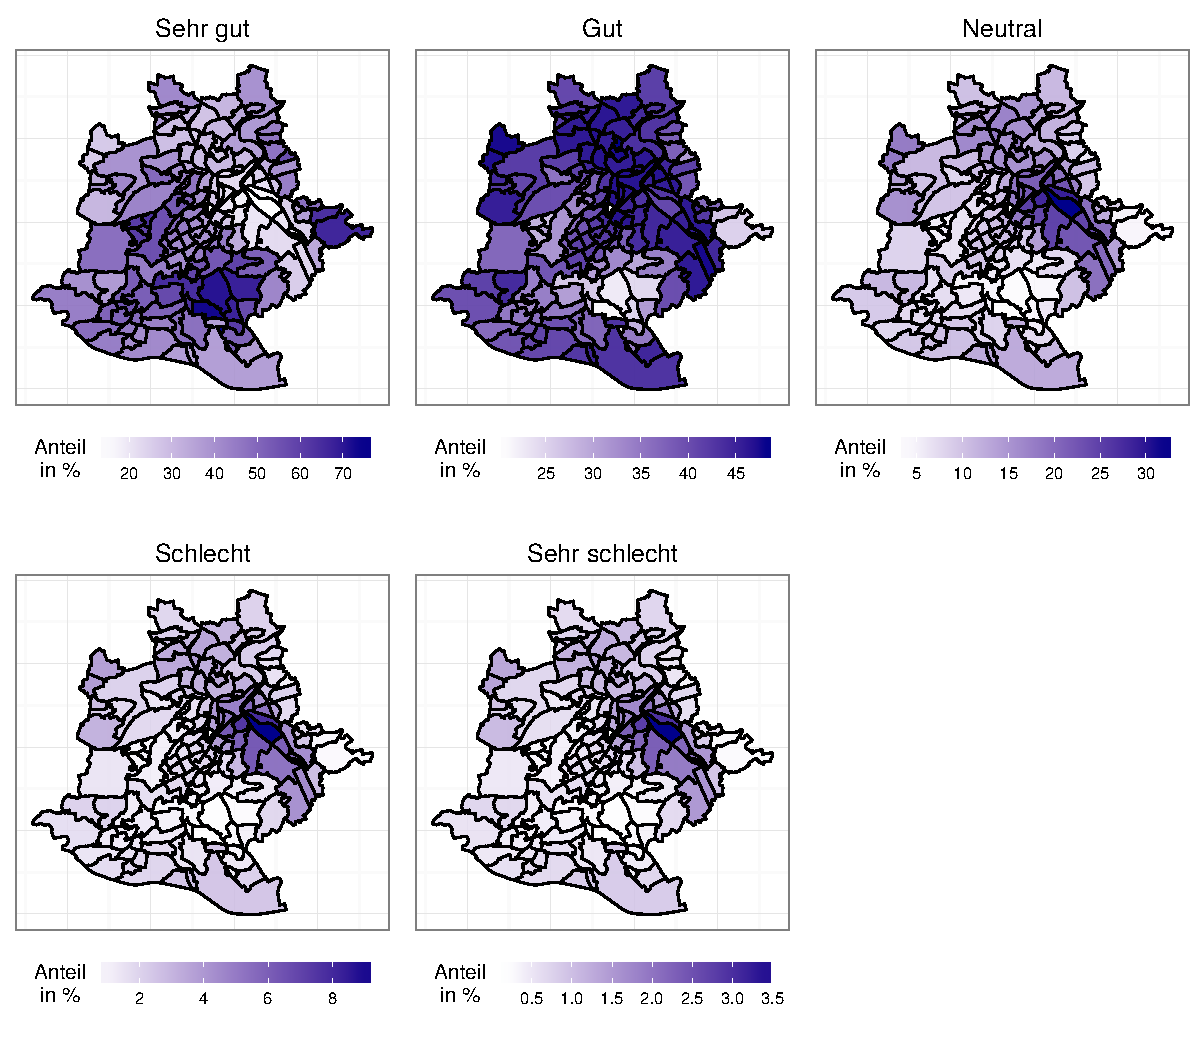
\includegraphics[scale=0.8]{Pictures/BWohnExtra}
 \caption{Extrapolierte Anteile auf Stadtteilebene für die Bewertung der Wohngegend mit dem besten Modell.}
 \label{WohnExtra}
 \end{center}
\end{figure}

\clearpage
\section{Diskussion}
Die Anzahlen der Beobachtungen in den Dateien sind sehr Unterschiedlich. Die Umfrage mit der die Modelle für die Hochrechnung parametrisiert wurden repräsentieren gerade 0,05\% der Grundgesamtheit. Die Dateien zur Extrapolation sind hingegen relativ nah an dieser Grundgesamtheit (82,0 bzw. 66,3\%). Bei der Interpretation der Ergebnisse muss also berücksichtigt werden, dass die Anzahl der befragten Personen deutlich geringer ist die Anzahl der Personen mit der die Extrapolation durchgeführt werden. Bei der relativ geringen Anzahl an Regressionsparametern (Tabellen \ref{ParameterTabS213spat}, \ref{ParameterTabS212spat} und \ref{ParameterTabW5spat}) ist die absolute Beobachtungsanzahl der Parametrsierungsdatei jedoch ausreichend. Zudem ersichtlich ist, dass jede Variablenausprägung ausreichend Beobachtungen enthält (Abbildungen \ref{endogene} und \ref{exogen_parametrisierungsdatensatz}). Selbst die seltensten Variablenausprägungen \textit{schlecht} und \textit{sehr schlecht} der Bewertung der Wohngegend zeigen jeweils genügend Beobachtungen. Es deutet also alles darauf hin, dass die Beobachtungen der Parametrisierungsdatei ausreichend sind, um ein stabiles Modell für die Extrapolation zu erstellen. Die Extrapolationsdateien selbst umfassen auch nicht die gesamte Grundgesamtheit. Im Auszug aus dem Melderegister beispielsweise fehlen Jugendliche unter 18 sowie Bewohner von Altersheimen. Da diese Dateien aber jeweils sehr viel der Grundgesamtheit abdecken, kann angenommen werden, dass die Aussagen, die aus diesen Daten abgeleitet werden für die Grundgesamtheit gültig sind.

\subsection{Schrittweiser AIC Vergleich}
\textcolor{red}{wir könnten Schrittweiser AIC Vergleich umbenennen in 'Kovariablenauswahl'}
Das AIC bildet eine gute Basis, um die geeignete Kovariablenkombination zu identifizieren, da es einen Kompromiss zwischen Anpassung und Komplexibilität sucht \cite{Akaike1981}. Das AIC ist geeignet um Rangfolgen von Modellen zu erstellen, also die relative Vorteilhaftigkeit eines Modelles gegenüber anderen zu quantifizieren. Das AIC sagt jedoch nicht über die absolute Qualität, also die Anpassungsgüte aus. Da von vornherein wenige Variablen für die Auswahl zur Verfügung standen und die Stichprobengröße relativ hoch war, sind in vielen Fällen alle Kovariablen in die Modelle eingeflossen.

\subsection{Modelle}
Der räumliche Effekt bringt in allen Modellen eine Verbesserung der Anpassung. Selbst in den Modellen, in denen der AIC sich durch den räumlichen Glättungsterm nicht verändert, kann von einer Verbesserung des Modells durch den räumlichen Effekt ausgegangen werden. Da die Modellkomplexibilität sich durch den räumlichen Effekt erhöht hat, impliziert ein unverändertes AIC eine bessere Modellanpassung. Da die Geodaten, die für die räumliche Komponente notwendig sind, in allen Dateien einfach verfügbar sind, gibt es keinen Grund auf diese Information im Modell zu verzichten.\\
Die univariaten Parameter haben relativ starken Einfluss auf die Ablehnungswahrscheinlichkeit. Bei der genaueren Betrachtung der räumlichen Effekte (Abbildung \ref{rEffS21}) zeigt sich jedoch, dass der räumliche Effekt sich ebenfalls auf die Ablehnungswahrscheinlichkeit auswirkt. Es gibt einen klaren räumlichen Trend in den Daten, wenngleich dieser in Relation zu den sozioökonomischen Kovariablen relativ schwach ausgeprägt ist. Die Meinung eines Bürgers zu Stuttgart 21 hängt also eindeutig auch von der Lage seiner Wohnung ab. In erster Linie ist die Meinung jedoch von den sozioökonomischen Kovariablen bestimmt (Abbildung \ref{GKParam}). Die Wahl des räumlichen Effektes ist dabei zweitrangig. Die Änderung der Parameterausprägung von Nord nach Süd ist stetig und nur sehr gering ausgeprägt. Der kontinuierliche räumliche Effekt liefert daher praktisch die gleichen Informationen wie der diskrete Trend auf Stadtbezirksebene. Die höhere Auflösung auf Stadtteilebene liefert nur im Süden zusätzliche Informationen. Diese hohe Auflösungsebene, die eine Vielzahl zusätzlicher Modellparameter mit sich bringt, scheint also nicht sinnvoll zu sein. Die Interpretation der Modelleffekte ergibt also, wie die AIC-Betrachtung (Tabelle \ref{stepAIC}), dass die beiden geoadditiven Modelle mit stetigem und diskretem räumlichen Trend auf Stadtbezirksebene für die Prognose der Meinung zu Stuttgart 21 gleichwertig und, dass das Modell auf Stadtteilebene nachrangig ist.\\
Der Bahnhof liegt an der nördlichen Grenze des Stadtviertels \textit{Mitte}, also ziemlich genau auf der Konturlinie, die den Übergang von \textit{Zustimmung} zu \textit{Ablehnung} markiert. Bürger, die südlich des Bahnhofs wohnen zeigen demnach eine höhere Ablehnungswahrscheinlichkeit als Bürger aus der nördlichen Hälfte Stuttgarts.\\
Die Wohnzufriedenheit hängt sehr viel stärker von der Lage der Wohnung ab als von den sozioökonomischen Kovariablen. Da die räumliche Lage bereits einen sehr hohen Erklärungsgehalt hat, sind deshalb weniger Kovariablen erforderlich als es bei der Meinung zu Stuttgart 21 der Fall ist. Umso wichtiger ist folglich die Auswahl des geeigneten räumlichen Effektes. Nach visueller Einschätzung ist die Auflösung des diskreten Effekts auf Stadtbezirksebene nicht hoch genug um das komplexe räumliche Muster zu beschreiben. Das Modell auf Stadtteilebene erscheint hingegen zu komplex zu sein, da insbesondere im Zentrum sehr kleinflächige Strukturen mit zum Teil sehr unterschiedlichen Parameterausprägungen zu sehen sind. Der kontinuierliche Effekt ist offensichtlich ein Kompromiss zwischen den beiden diskreten Trends. Die kleinräumig unterschiedlichen Parameterausprägungen, wie sie z.B. im Nordosten zu sehen sind werden durch das kontinuierliche Modell dargestellt. Dabei schwanken die Parameter, insbesondere im Zentrum, weniger stark als beim Modell auf Stadtteilebene. Die Analyse der AIC (Tabelle \ref{stepAIC}) unterstreicht diese visuellen Einschätzungen.

\subsection{Reklassifizierung}
Die Reklassifizierung bildet das erste absolute Modellqualitätskriterium. Es zeigt sich, wie zuvor angedeutet, dass die geoadditiven Modelle bei allen drei Ausprägungen der Response-Variablen vorteilhaft gegenüber reinen GAM sind. Sowohl bei zwei- als auch bei dreikategorialer Response bei der Modellierung der Meinung zu Stuttgart 21 bestätigen sich die Ergebnisse aus der visuellen Interpretation sowie der AIC Analyse (Tabelle \ref{evalS21}). Die Berücksichtigung des räumlichen Trends verbessert die Schätzgenauigkeit. Dabei sind der kontinuierliche und der diskrete räumliche Trend auf Bezirksniveau gleichwertig. Der räumliche Trend auf Stadtteilebene schneidet schlechter ab. Die Ergebnisse der Reklassifizierung der Wohnzufriedenheit (Tabelle \ref{evalB}) fügen sich ebenfalls in die Vorüberlegungen ein. Das diskrete Modell erweist sich als vorteilhaft. Bemerkenswerterweise ist der durchschnittliche Anteil korrekt reklassifizierter Beobachtungen bei dem geoadditiven Modell mit diskreten räumlichem Trend Modell auf Stadtteilebene schlechter als bei den Modellen mit sozioökonomischen Kovariablen und dem alleinigen räumlichen Trend. Dies zeigt, wie die visuelle Analyse bereits andeutete, dass die Parameteranzahl deutlich zu hoch ist, das Modell also überangepasst ist.

\subsection{Kreuzvalidierung}
Die Kreuzvalidierung ist eine sehr computerintensive Berechnung. Daher wurden die ohnehin nicht vielversprechenden Modelle ohne räumlichen Trend und nur mit räumlichen Trend bei dieser Analyse nicht mehr berücksichtigt. Zunächst ist zu bemerken, dass der durchschnittliche korrekt klassifizierte Anteil der Beobachtungen \textit{out-of-sample} (Tabellen \ref{KreuzM} und \ref{KreuzBew}) den korrekt reklassifizierten Anteil der Beobachtungen (Tabellen \ref{evalS21} und \ref{evalB}) stets sehr ähnelt. Abweichungen sind als Zufall zu interpretieren. Dies deutet darauf hin, dass die Modelle sehr robust sind.
In dieser Betrachtungsebene zeigt sich auch erstmals, dass die guten Ergebnisse bei der Reklassifizierung und der Kreuzvalidierung in erster Linie durch die korrekte Schätzung der wahrscheinlichsten Gruppen zurückzuführen sind. Die weniger wahrscheinlichen Gruppen werden praktisch nie korrekt reklassifiziert. Diese individuelle Fehleinschätzung spielt für die in dieser Arbeit angestrebte räumliche Extrapolation jedoch keine Rolle, da hierzu mittlere Anteile auf regionaler Ebene gebildet werden.

\subsection{Kleinräumige Extrapolation}

\subsubsection{Validierung}
Da Stimmanteile zur Volksabstimmung zu Stuttgart 21 vorlagen, konnte das Ergebnis der räumlichen Extrapolation mit dem tatsächlichen Ergebnis vergleichen werden.
Da in dieser Volksabstimmung nur Informationen zu zwei Klassen verfügbar sind, wurde erwartet, dass das zwei Klassenmodell die beiden Kategorien besser prognostiziert. Die Analyse des MSE und der Überdeckungswahrscheinlichkeit ergab jedoch, dass das dreikategoriale zur Prognose der \textit{Zustimmung} deutlich besser geeignet ist. Bei einer Volksabstimmung ist eine \textit{neutrale} Haltung keine Option. Daher kann das sehr genau eingeschätzte Ergebnis der \textit{Zustimmung} genutzt werden, um den voraussichtlichen \textit{Ablehnungsanteil} als $100\% -\textit{Zustimmung}$ zu berechnen. Anders ausgedrückt könnten die Ergebnisse dieser Arbeit auch so interpretiert werden, dass Bürger, die bei der Bürgerumfrage bei der Frage zur Meinung zu Stuttgart 21 mit \textit{neutral} geantwortet haben bei der Volksabstimmung, bei der es kein \textit{neutral} gibt, überwiegend gegen das Projekt gestimmt haben oder nicht zur Wahl gegangen sind.\\
Die guten Validierungsergebnisse geben demnach Hinweis, dass die dreikategorialen geoadditiven Modelle mit kontinuierlichem sowie diskretem räumlichen Trend auf Bezirksebene sehr gut für die Prognose der Meinung zu Stuttgart 21 geeignet sind. Da das Modell zur Wohnzufriedenheit auf selber Datengrundlage erstellt wurde und auch methodisch dem Stuttgart-21-Modell entspricht, kann angenommen werden, dass auch mit diesem Wohnzufriedenheits-Modell sehr genaue Prognosen erstellt werden können. Die positive Evaluation der Ergebnisse lässt zudem den Schluss zu, das auch die Modellelemente valide sind. Die Sekundärinformationen, die sich beispielsweise aus den Modellkoeffizienten interpretieren lassen, sind somit ebenfalls validiert.\\
Die Modelle mit zweikategorialer Response schneiden beim Vergleich der MSE und der Über\-deckungs\-wahrscheinlichkeit schlechter ab. An dieser Stelle können also auch diese Modelle für die kleinräumige Extrapolation ausgeschlossen werden.\\
Bei dem Vergleich darf nicht außer acht gelassen werden, dass der angenommene wahre Wert nicht der tatsächliche wahre Wert der Grundgesamtheit der Stichprobe ist. Die Volksabstimmungsergebisse sind Hilfsvariablen für die wahren Anteile der unbekannten Grundgesamtheit. Insbesondere da bei der Volksabstimmung keine \textit{neutrale} Klasse erfasst wurde und weil die Volksabstimmung zu einem anderen Zeitpunkt stattfand als die Erhebung der Parametrisierungsstichprobe (siehe \textit{Material und Methoden}). Die Berechneten MSE sind entsprechend als Hilfsvariablen für die Überprüfung der Modellqualität zu interpretieren. Anhand der MSE lässt sich erkennen, dass unsere Modelle in der Lage sind ein sinnvolles und nachvollziehbares Ergebnis zu produzieren. Ob die Modelle den wahren Wert der Grundgesamtheit tatsächlich approximieren lässt sich mit der Methode jedoch nicht klären.

\subsubsection{Prognose}
Die beiden Dateien an der die Modelle angewendet wurden zeichnen sich durch einen sehr großen Stichprobenumfang aus. Dennoch muss beachtet werden, dass sie jeweils nicht die gesamte Bevölkerung Stuttgarts, sondern nur einen großen Teil der Bevölkerung, enthalten. Die abgeleiteten Ergebnisse aus diesen Extrapolationsdateien werden als Ergebnis für die Grundgesamtheit, also für alle Bürger Stuttgarts, interpretiert. Dies wird aufgrund dieser hohen Stichprobenumfänge als unproblematisch angesehen.\\
Die Prognoseintervalle der Anteilsschätzung durch Extrapolation sind relativ breit (Abbildungen \ref{S21Alle} und \ref{WAlle}). Durch eine Erhöhung des Stichprobenumfangs bei der Parametriseierungsstichprobe könnte diese Unsicherheit vermutlich reduziert werden. Da alle Prüfungen dieser Arbeit jedoch auf Konsistenz der Punktschätzungen hindeuten, kann davon ausgegangen werden, dass es sich um eine nicht-systematische, symmetrische Unsicherheit um die Punktschätzung handelt. Eine Erhöhung des Stichprobenumfangs würde demnach voraussichtlich zu einer Verkleinerung der Vertrauensbereiche, jedoch nicht zu einer merklichen Veränderung der Punktschätzungen führen.\\
Für eine unbekannte Grundgesamtheit lässt sich nur schwer sagen, welches der Modell letztlich die beste Schätzung liefert. Die Ergebnisse der Extrapolation ordnen sich jedoch in alle Vorüberlegungen ein. Bei der Meinung zu Stuttgart 21 (Abbildung \ref{S21Alle}) liegen die Modelle mit kontinuierlichem und diskretem räumlichen Term auf Stadtbezirksniveau gleichauf. Sie liefern, in Verbindung mit allen vorhergegangenen Validierungsergebnissen, voraussichtlich die beste Schätzung. Im Falle der Modellierung der Wohnzufriedenheit (Abbildung \ref{WAlle}) scheint sich das geoadditive Modell mit kontinuierlicher räumlicher Information deutlich abzusetzen, obwohl das Modell mit den Stadtbezirksinformationen schmalere Prognoseintervalle liefert. Es hebt sich relativ stark von den Schätzungen durch die anderen Modelle ab und schneidet bei den vorhergegangenen Validierungen stets am besten ab. Es war zu erwarten, dass das diskrete geoadditive Modell auf Bezirksebene die schmalsten Prognoseintervalle liefert. Die Analyse der Modelleffekte zeigte, dass die relativ grobe räumliche Einteilung dem Datensatz die Variabilität der Rohdaten nicht widerspiegeln kann (Abbildung \ref{rEffW}). Durch Anwendung dieses Modells werden die Ergebnisse also künstlich homogenisiert und die wahre Datenvariabilität somit nicht widergespiegelt (\textit{Underfitting}). Aus diesen Gründen wurden für die kleinräumige Extrapolation für die Stadtviertel \textcolor{red}{sind das jetzt bezrike oder teile?} (Abbildungen \ref{S21Extra} und \ref{WohnExtra}) für beide Fragestellungen die geoadditiven Modelle mit kontinuierlichem räumlichen Effekt verwendet.\\
Im Bereich der Stadtteile \textit{Benzviertel} und \textit{Wasen} scheint ein Hot-Spot der Wohnunzufriedenheit zu liegen. Bei der Interpretation dieses Sachverhalts muss beachtet werden, dass es sich bei den beiden Stadtteilen um sehr dünn besiedelte Stadtteile handelt bei denen in der Parametrisierungsstichprobe jeweils keine einzige Beobachtung zu finden ist. Der Prädiktorparameter des räumlich Trends dieser beiden Stadtteile basiert also nur auf der Glättung durch die Beobachtungen der Nachbarstadtteile und nicht auf Beobachtungen aus den Stadtteilen selbst.

%============================================== Conlcusion =========================================================%
\newpage
\section{Fazit}
Wir haben gezeigt, dass es möglich ist die Einflüsse, die bei den Bürgern Stuttgarts zu einer Entscheidung der beiden einleitenden Fragen führt, zu modellieren. Zudem konnte anhand verschiedener statistischer Gütemaße die Eignung unterschiedlicher Modellierungsansätze, die sich in Bezug auf ihre räumlichen Effekte, Verteilung der Response-Variablen und sozioökonomischen Variablen unterschieden, untersucht werden. Die einleitenden Fragestellungen ließen sich demnach über die Extrapoliation zufriedenstellend beantworten.\\
Das Modell, das sich am besten für die Modellierung der Meinung zu Stuttgart 21 eignet besteht aus den Kovariablen \textit{Geschlecht}, \textit{Nationalität}, \textit{Familienstand}, \textit{Anzahl der im Haushalt lebenden Personen}, \textit{Altersklasse der Befragten}, der Wechselwirkung aus \textit{Altersklasse} und  \textit{Personenzahl im Haushalt} sowie einem diskreten räumlichen Trend. Die geordnete dreikategoriale Response-Variable hat sich gegenüber der binären Variable als vorteilhaft erwiesen. Die Parameter, die die Bewertung der Wohngegend am besten beschreiben sind \textit{Nationalität}, \textit{Personenzahl im Haushalt}, \textit{Altersklasse} sowie der kontinuierliche räumliche Effekt. Es zeigt sich, dass sich die Hochrechnungen durch die Extrapolation von der einfachen deskriptiven Auswertung der Stichprobe abheben. Es ist anzunehmen, dass die einfache deskriptive Auswertung verzerrt ist, da die Beobachtungen nach Gruppen und Region teils sehr unterschiedlich in den Rohdaten repräsentiert sind.\\
Für gesamt Stuttgart bedeuten die Ergebnisse, dass 51\% der Bürger eine \textit{positive} Meinung zu Stuttgart 21, 21\% eine \textit{neutrale} Meinung und 28\% eine negative Meinung zu Stuttgart 21 haben. Wobei eine Validierung mit den tatsächlichen Ergebnissen der Volksabstimmung gezeigt hat, dass der Großteil der Personen mit \textit{neutraler} Meinung bei der Volksabstimmung womöglich eher gegen das Projekt gestimmt hat. Bei der Modellierung zur Bewertung der Wohngegend ergab sich, dass 43\% der Bürger Stuttgarts eine \textit{sehr gute} und 41\% eine \textit{gute} Meinung ihrer Wohngegend haben. 13\% Bewerten ihre Wohngegend \textit{neutral}. \textit{Schlechte} und \textit{sehr schlechte} sind mit 3\% bzw. 1\% deutlich seltener.\\
In der Parametrsierungsstichprobe sind noch weitere Variablen enthalten, die für die Modellparametrisierung zur Verfügung stehen. Von diesen birgt insbesondere das \textit{monatliche Nettoeinkommen} ein hohes Potenzial. Im Laufe der Modellierung stellte sich heraus, dass das \textit{monatliche Nettoeinkommen} einen hohen Erklärungsgehalt hat. Wen es gelingt, diese Variable in einem der Hochrechnungsdateien zu generieren oder zu approximieren, könnt dies die Schätzgenauigkeit nochmals recht deutlich erhöhen.
Außerdem wäre es sinnvoll model avereging Ansätze zu verfolgen, z.B. über gewichtete AIC \cite{WAIC}. Dabei werden die Schätzer und Standardfehler aus den Modellen kombiniert, wodurch Unsicherheiten in der Modellwahl direkt in die Parameterschätzer mit einfließen können\cite{ModelAver}.\\
Diese Arbeit zeigt beispielhaft die Durchführung einer kleinräumigen Extrapolation inklusive der Interpreation der einzelnen Modellkomponenten. es sind sicherlich auch noch weitere Auswertungen und Interpretationen mit den Daten und Modellen dieser Arbeit möglich. So könnte beispielsweise auch eine andere nicht-räumliche Aggregationsebene interessant sein. Die Daten dieser Arbeit könnten z. B. genutzt werden, um die Meinungen nach weiteren Variablen hochzurechnen. Denkbar wäre beispielsweise der Vergleich der Wohnzufriedenheit von Bürgern mit Wohneigentum mit Bürgern die zur Miete wohnen.\\
\clearpage


%============================================ References ===========================================================%
\addcontentsline{toc}{section}{\numberline{}Literatur}
\bibliographystyle{apalike}
\bibliography{LiteraturStuttgart.bib} 

%\section{References}
%\renewcommand{\section}[2]{}
%\addcontentsline{toc}{section}{References}
%\renewcommand{\bibname}{4 References}
%\phantomsection
%\addcontentsline{toc}{section}{References}




\clearpage

%============================================== Appendix ============================================================%
%\appendix
%\pagestyle{Myheadings}
\chead{ANHANG}
%\pagestyle{}
%\section{$A^{-1}$ Appendix}
%\setcounter{secnumdepth}{0}

\begin{appendix}

\section*{Anhang}
\addcontentsline{toc}{section}{\numberline{}Anhang}

\begin{figure}[h]
 \begin{center}
 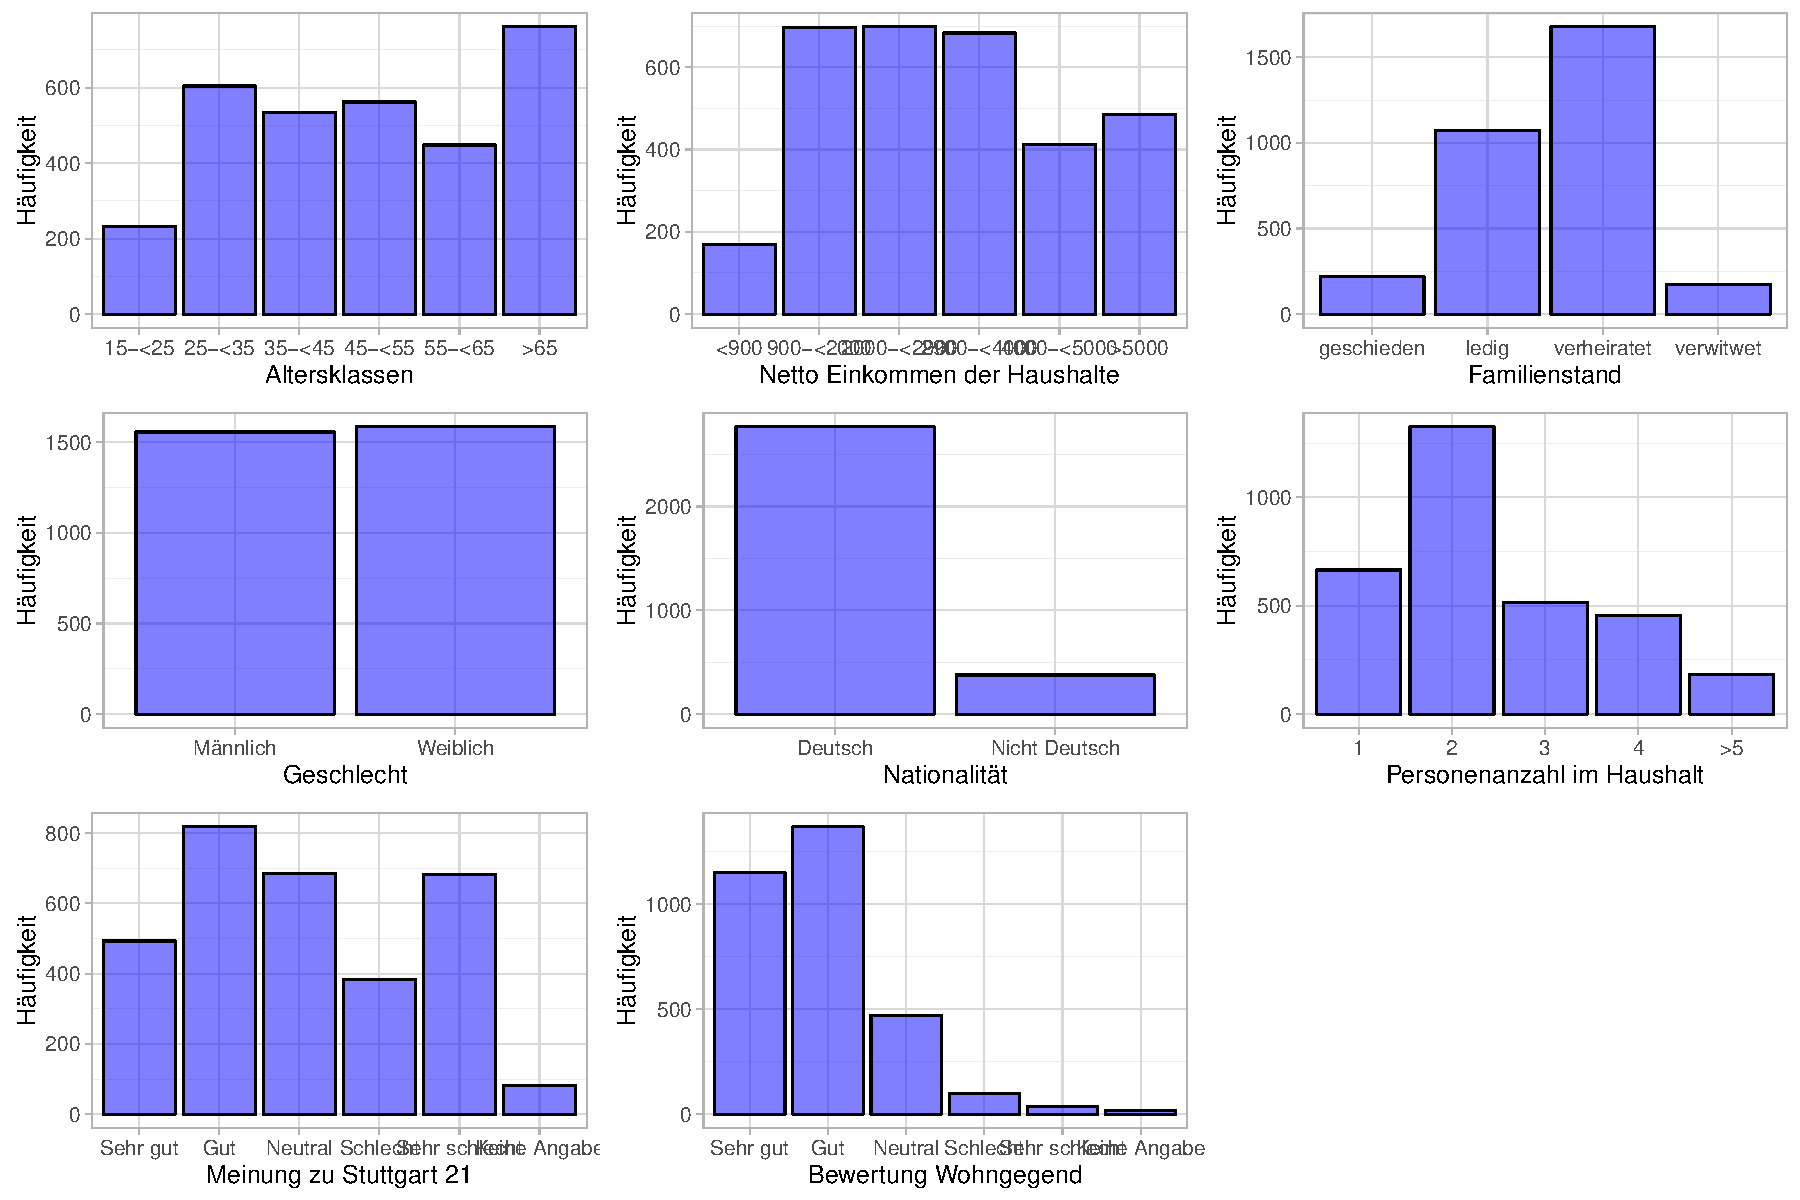
\includegraphics[scale=0.8]{Pictures/BarData}
 \caption{Häufigkeit der Kategorienausprägungen der exogenen Variablen in der Parameterisierungsstichprobe.}
 \label{exogen_parametrisierungsdatensatz}
 \end{center}
\end{figure}


\begin{figure}[h]
 \begin{center}
 
\includegraphics[scale=0.8]{Pictures/BWohn}
 \caption{Anteile der Bewertung der Wohngegend nach Stadtbezirken.}
 \label{BWohn}
 \end{center}
\end{figure}

\begin{figure}[h]
 \begin{center}
 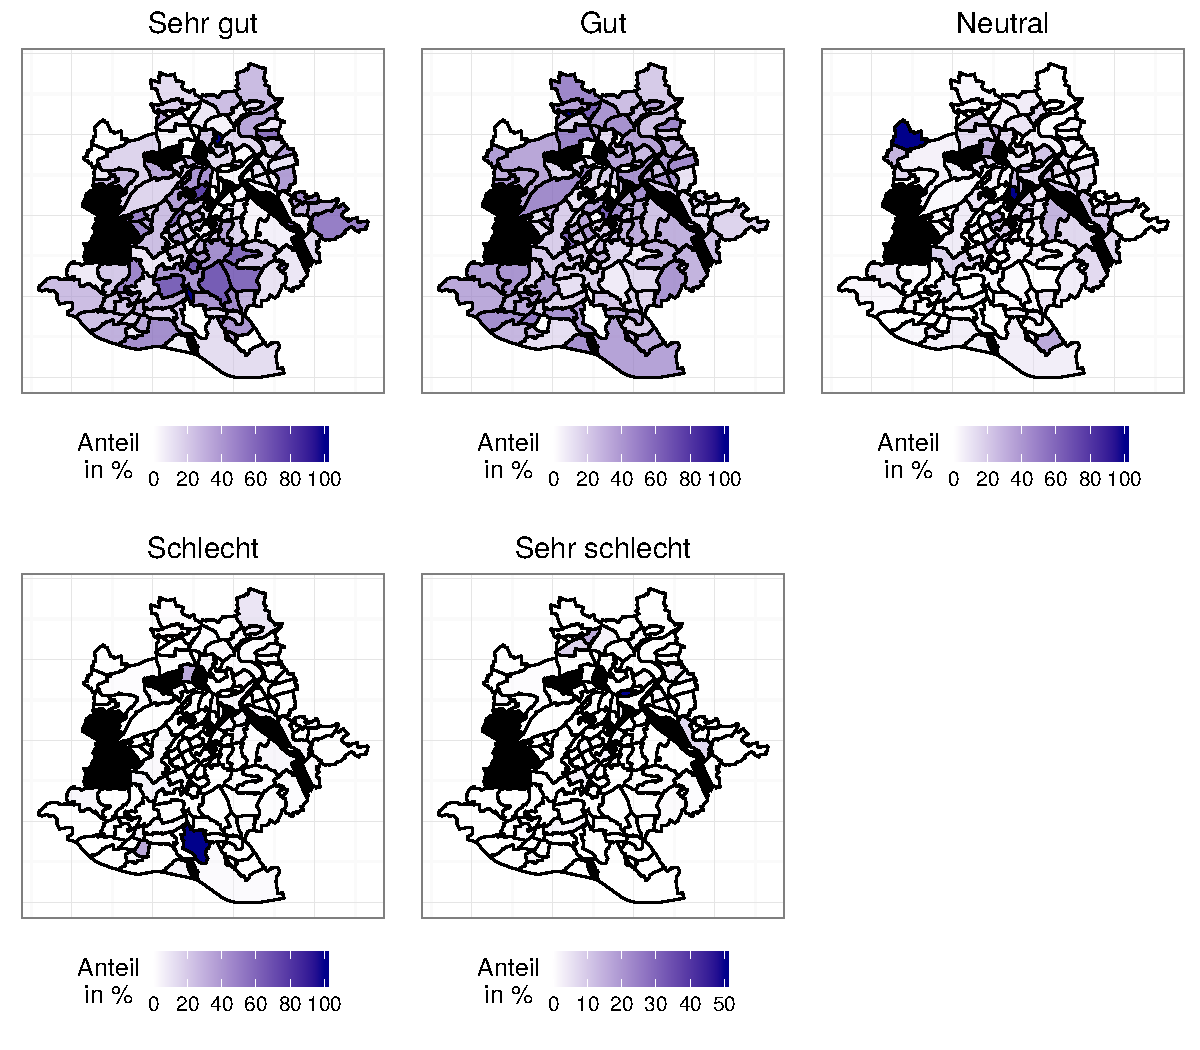
\includegraphics[scale=0.8]{Pictures/SWohn}
 \caption{Anteile der Bewertung der Wohngegend nach Stadtteilen.}
 \label{SWohn}
 \end{center}
\end{figure}

%\begin{figure}[h]
% \begin{center}
% 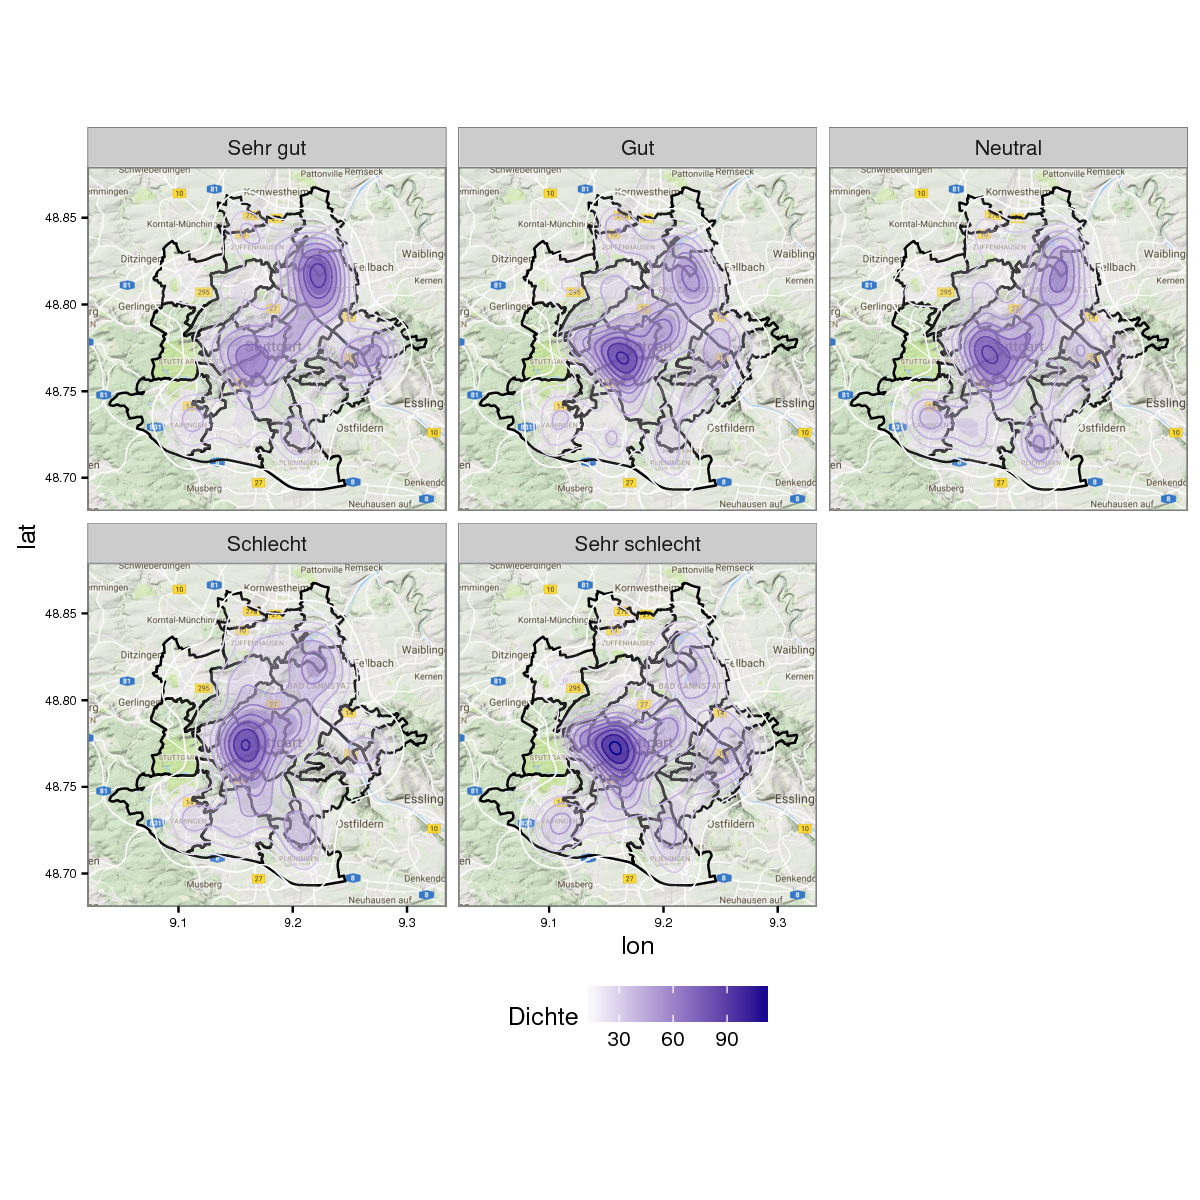
\includegraphics[scale=0.8]{Pictures/XYStuttgart5}
% \caption{Gauß Krüger Informationen Stuttgart 21 (2)}
% \label{endogene}
% \end{center}
%\end{figure}


\clearpage

% Table created by stargazer v.5.2 by Marek Hlavac, Harvard University. E-mail: hlavac at fas.harvard.edu
% Date and time: Di, Sep 27, 2016 - 21:39:45
\begin{table}[h] \centering 
  \caption{Zusammenfassung der drei geoadditiven Modelle zur Modellierung der Meinung zu Stuttgart 21 mit dreikategorialer Response. (A): Kontinuierlicher räumlicher Trend, (B): Diskreter räumlicher Trend auf Stadtbezirksebene, (C): Diskreter räumlicher Trend auf Stadtteilebene.} 
  \label{ParameterTabS213spat} 
\begin{tabular}{@{\extracolsep{5pt}}lccc} 
\\[-1.8ex]\hline 
\hline \\[-1.8ex] 
 & \multicolumn{3}{c}{\textit{Abhängige Variable:}} \\ 
\cline{2-4} 
\\[-1.8ex] & \multicolumn{3}{c}{Meinung zu Stuttgart 21} \\ 
\\[-1.8ex] & (A) & (B) & (C)\\ 
\hline \\[-1.8ex] 
 Geschlecht: weiblich & 0.524$^{***}$ & 0.508$^{***}$ & 0.538$^{***}$ \\ 
  & (0.070) & (0.069) & (0.069) \\ 
  & & & \\ 
 Nationalität: nicht deutsch & $-$0.445$^{***}$ & $-$0.472$^{***}$ & $-$0.454$^{***}$ \\ 
  & (0.110) & (0.109) & (0.110) \\ 
  & & & \\ 
 Familienstand: ledig & 0.090 &  & 0.084 \\ 
  & (0.159) &  & (0.159) \\ 
  & & & \\ 
 Familienstand: verheiratet & $-$0.176 &  & $-$0.189 \\ 
  & (0.151) &  & (0.152) \\ 
  & & & \\ 
 Familienstand: verwitwet & $-$0.356$^{*}$ &  & $-$0.413$^{**}$ \\ 
  & (0.207) &  & (0.208) \\ 
  & & & \\ 
 Personenzahl im Haushalt & $-$0.340$^{***}$ & $-$0.369$^{***}$ & $-$0.348$^{***}$ \\ 
  & (0.060) & (0.021) & (0.061) \\ 
  & & & \\ \hline
 s(X,Y) & $*$ &  &  \\ 
  & & & \\ 
 s(Stadtbezirk) &  & $*$ &  \\ 
  & & & \\ 
 s(Stadtteil)&  &  & $*$ \\ 
  & & & \\ 
 s(Personenzahl im Haushalt, Altersklasse Befragter) & $***$ & $***$ & $***$  \\ 
  & & & \\ 
 s(Altersklasse Befragter) & $***$ & $***$  & $***$ \\ 
  & & & \\ 
 Konstante & 0.000 & 0.000 & 0.000 \\ 
  & (0.000) & (0.000) & (0.000) \\ 
  & & & \\ 
\hline \\[-1.8ex] 
Beobachtungen & 3,062 & 3,062 & 3,093 \\ 
Log Likelihood & $-$3,186.494 & $-$3,187.330 & $-$3,210.754 \\ 
UBRE & 3,197.650 & 3,195.841 & 3,219.511 \\ 
\hline 
\hline \\[-1.8ex] 
\textit{Sign. Codes:}  & \multicolumn{3}{r}{$^{*}$p$<$0.1; $^{**}$p$<$0.05; $^{***}$p$<$0.01} \\ 
\end{tabular} 
\end{table} 

% Table created by stargazer v.5.2 by Marek Hlavac, Harvard University. E-mail: hlavac at fas.harvard.edu
% Date and time: Di, Sep 27, 2016 - 21:54:03
\begin{table}[!htbp] \centering 
  \caption{Zusammenfassung der drei geoadditiven Modelle zur Modellierung der Meinung zu Stuttgart 21 mit zweikategorialer Response. (A): Kontinuierlicher räumlicher Trend, (B): Diskreter räumlicher Trend auf Stadtbezirksebene, (C): Diskreter räumlicher Trend auf Stadtteilebene.} 
  \label{ParameterTabS212spat} 
\begin{tabular}{@{\extracolsep{5pt}}lccc} 
\\[-1.8ex]\hline 
\hline \\[-1.8ex] 
 & \multicolumn{3}{c}{\textit{Abhängige Variable:}} \\ 
\cline{2-4} 
\\[-1.8ex] & \multicolumn{3}{c}{Meinung zu Stuttgart 21} \\ 
\\[-1.8ex] & (A) & (B) & (C)\\ 
\hline \\[-1.8ex] 
 Geschlecht: weiblich & 0.644$^{***}$ & 0.646$^{***}$ & 0.642$^{***}$ \\ 
  & (0.087) & (0.087) & (0.088) \\ 
  & & & \\ 
 Nationalität: nicht deutsch & $-$0.721$^{***}$ & $-$0.723$^{***}$ & $-$0.757$^{***}$ \\ 
  & (0.154) & (0.154) & (0.156) \\ 
  & & & \\ 
 Familienstand: ledig & 0.022 & 0.037 & 0.102 \\ 
  & (0.191) & (0.191) & (0.196) \\ 
  & & & \\ 
 Familienstand: verheiratet & $-$0.333$^{**}$ & $-$0.316$^{*}$ & $-$0.215 \\ 
  & (0.170) & (0.170) & (0.186) \\ 
  & & & \\ 
 Familienstand: verwitwet & $-$0.244 & $-$0.234 & $-$0.431$^{*}$ \\ 
  & (0.243) & (0.243) & (0.251) \\ 
  & & & \\ 
   Personenzahl im Haushalt &  &  & $-$0.155$^{**}$ \\ 
  &  &  & (0.075) \\ 
    & & & \\ \hline
 s(X,Y) & $*$ &  &  \\ 
  & & & \\ 
 s(Stadtbezirk) &  & $**$ &  \\ 
  & & & \\ 
 s(Stadtteil) &  &  & $**$ \\ 
  & & & \\ 
 s(Personenzahl im Haushalt, Altersklasse Befragter) &  &  &  \\ 
  & & & \\ 
 s(Altersklasse Befragter) & $***$ & $***$ & $***$ \\ 
  & & & \\ 
 Konstante & $-$0.283$^{*}$ & $-$0.298$^{*}$ & 0.000 \\ 
  & (0.171) & (0.171) & (0.000) \\ 
  & & & \\ 
\hline \\[-1.8ex] 
Beobachtungen & 2,377 & 2,377 & 2,394 \\ 
Adjusted R$^{2}$ & 0.070 & 0.071 & 0.078 \\ 
Log Likelihood & $-$1,556.448 & $-$1,556.146 & $-$1,537.527 \\ 
UBRE & 1,563.538 & 1,561.176 & 1,544.394 \\ 
\hline 
\hline \\[-1.8ex] 
\textit{Sign. Codes:}  & \multicolumn{3}{r}{$^{*}$p$<$0.1; $^{**}$p$<$0.05; $^{***}$p$<$0.01} \\ 
\end{tabular} 
\end{table} 


% Table created by stargazer v.5.2 by Marek Hlavac, Harvard University. E-mail: hlavac at fas.harvard.edu
% Date and time: Di, Sep 27, 2016 - 22:16:06
\begin{table}[h] \centering 
  \caption{Zusammenfassung der drei geoadditiven Modelle zur Modellierung der Wohnzufriedenheit mit dreikategorialer Response. (A): Kontinuierlicher räumlicher Trend, (B): Diskreter räumlicher Trend auf Stadtbezirksebene, (C): Diskreter räumlicher Trend auf Stadtteilebene.} 
  \label{ParameterTabW5spat} 
\begin{tabular}{@{\extracolsep{5pt}}lccc} 
\\[-1.8ex]\hline 
\hline \\[-1.8ex] 
 & \multicolumn{3}{c}{\textit{Abhängige Variable:}} \\ 
\cline{2-4} 
\\[-1.8ex] & \multicolumn{3}{c}{Bewertung Wohngegend} \\ 
\\[-1.8ex] & (A) & (B) & (C)\\ 
\hline \\[-1.8ex] 
 Nationalität: nicht deutsch & 0.289$^{***}$ & 0.359$^{***}$ &  \\ 
  & (0.107) & (0.106) &  \\ 
  & & & \\ 
 Personenzahl im Haushalt & $-$0.043 & $-$0.047 &  \\ 
  & (0.032) & (0.032) &  \\ 
  & & & \\ 
 Familienstand: ledig &  &  & 0.021 \\ 
  &  &  & (0.157) \\ 
  & & & \\ 
 Familienstand: verheiratet &  &  & 0.561$^{***}$ \\ 
  &  &  & (0.149) \\ 
  & & & \\ 
 Familienstand: verwitwet &  &  & $-$0.286 \\ 
  &  &  & (0.204) \\ 
  & & & \\ 
 Geschlecht: weiblich &  &  & $-$0.318$^{***}$ \\ 
  &  &  & (0.067) \\ \hline
   & & & \\ 
 s(X,Y) & $***$ &  &  \\ 
  & & & \\ 
 s(Stadtbezirk)&  & $***$ &  \\ 
  & & & \\ 
 s(Stadtteil) &  &  & $***$ \\ 
  & & & \\ 
 s(Altersklasse Befragter) & $***$ & $***$  & $***$ \\ 
  & & & \\ 
 s(Personenzahl im Haushalt) &  &  & $***$ \\ 
  & & & \\ 
 Konstante & $-$0.339$^{***}$ & $-$0.357$^{***}$ & $-$0.271$^{*}$ \\ 
  & (0.084) & (0.083) & (0.143) \\ 
  & & & \\ 
\hline \\[-1.8ex] 
Beobachtungen & 3,127 & 3,127 & 3,398 \\ 
Log Likelihood & $-$3,520.997 & $-$3,583.264 & $-$4,120.775 \\ 
UBRE & 3,550.796 & 3,598.430 & 4,158.075 \\ 
\hline 
\hline \\[-1.8ex] 
\textit{Sign. Codes:}  & \multicolumn{3}{r}{$^{*}$p$<$0.1; $^{**}$p$<$0.05; $^{***}$p$<$0.01} \\ 
\end{tabular} 
\end{table} 

\end{appendix}
\clearpage
\pagestyle{plain}
%\phantomsection
%\addcontentsline{toc}{section}{Eigenständigkeitserklärung}

%\section{Eigenständigkeitserklärung}

Hiermit versichere ich, dass ich die vorliegende Hausarbeit selbstständig verfasst und keine anderen als die angegebenen
Hilfsmittel benutzt habe. Alle wörtlich oder sinngemäß den Schriften anderer entnommenen Stellen
habe ich unter Angabe der Quellen kenntlich gemacht. Dies gilt auch für beigefügte Zeichnungen, Skizzen, bildliche
Darstellungen und dergleichen.\\
\\
Mir ist bewusst, dass ich mich im Falle einer unbeabsichtigten oder vorsätzlichen Missachtung durch den fehlerhaften
Umgang mit Quellen unter Umständen strafbar mache und die vorliegende Hausarbeit mit nicht ausreichend
bewertet wird.
\\
\\Göttingen, den
\\Unterschrift
\vspace*{4cm}
\\
Hiermit erlaube ich, dass meine Arbeit auf Betrug und falsche, sowie fehlende Zitate auch online geprüft wird.\\
\\
Mir ist bewusst, dass ich mich im Falle einer unbeabsichtigten oder vorsätzlichen Missachtung durch den fehlerhaften
Umgang mit Quellen unter Umständen strafbar mache und die vorliegende Hausarbeit mit nicht ausreichend
bewertet wird.
\\
\\Göttingen, den
\\Unterschrift
\clearpage


\end{document}
